\documentclass[
    a5paper,
    pagesize,
    11pt,
    bibtotoc,
    normalheadings,
    twoside,
    openany,
    chapterprefix,
    DIV=9
]{scrbook}

\usepackage[utf8]{inputenc}
\usepackage{tocloft}
\usepackage{mathtools}
\usepackage{amsfonts}
\usepackage{enumitem}
\usepackage{amsmath}
\usepackage{amsthm}
\usepackage{amssymb}
\usepackage[hmargin=2cm, vmargin=2.5cm]{geometry}
\usepackage{graphicx}
\usepackage{wrapfig}
\usepackage{parskip}
\usepackage{framed}
\usepackage{fancyhdr}
\usepackage{emptypage}
\usepackage{multicol}
\usepackage{imakeidx}
\usepackage[breaklinks]{hyperref}
\usepackage[capitalise, nameinlink]{cleveref}
\usepackage{crossreftools}

\usepackage[
    backend=bibtex,
    style=alphabetic,
    sorting=ynt
]{biblatex}

%=========== Path to images ==============
\graphicspath{{./images/}}

%============== Resources ================
\addbibresource{../AbstractAlgebra.bib}

%============ Redefinitions ==============
\let\oldemptyset\emptyset
\let\emptyset\varnothing

\let\totient\varphi

\renewcommand{\vert}{ \ \vline \ }
\newcommand{\vertalt}{ \ | \ }

\newcommand{\myref}[1]{\textbf{\crthypercref{#1}}}
\newcommand{\myreffigures}[1]{\textbf{\cref{#1}}}

%======== Theorem-Like Things ============
\newtheoremstyle{exercise-style}
    {-5pt}       % Space above
    {\topsep}    % Space below
    {}           % Font to use in exercise
    {0pt}        % Measure of space to indent
    {\bfseries}  % Name of the head font
    {.}          % Punctuation between head and body
    { }          % Space after theorem head; " " = normal inter-word space
    {\thmname{#1}\thmnumber{ #2}\textnormal{\thmnote{ (#3)}}}

\newtheorem{theorem}{Theorem}[section]
\renewcommand{\thetheorem}{\Roman{part}.\arabic{chapter}.\arabic{section}.\arabic{theorem}}

\newtheorem{conjecture}[theorem]{Conjecture}
\newtheorem{proposition}[theorem]{Proposition}
\newtheorem{definition}[theorem]{Definition}
\newtheorem{lemma}[theorem]{Lemma}
\newtheorem{corollary}[theorem]{Corollary}
\theoremstyle{definition}\newtheorem*{remark}{Remark}
\theoremstyle{definition}\newtheorem{example}[theorem]{Example}

\theoremstyle{exercise-style}\newtheorem{exercisehidden}{Exercise}[chapter]
\renewcommand{\theexercisehidden}{\Roman{part}.\arabic{chapter}.\arabic{exercisehidden}}

\theoremstyle{definition}\newtheorem{problem}{Problem}[chapter]
\renewcommand{\theproblem}{\Roman{part}.\arabic{chapter}.\arabic{problem}}

%============ Environments ===============
\newenvironment{exercise}
{\begin{framed}\noindent\begin{exercisehidden}}
{\end{exercisehidden}\end{framed}}

%=========== Custom Commands =============
\newcommand{\code}[1]{\texttt{#1}}  % Code block
\makeatletter\newcommand*{\rom}[1]{\Ifstr{#1}{0}{0}{\expandafter\@slowromancap\romannumeral #1@}}\makeatother  % Roman numeral

\newcommand{\lcm}{\mathrm{lcm}}  % Lowest common multiple function
\newcommand{\sgn}{\mathrm{sgn}}  % Signum function

\newcommand{\im}{\mathrm{im}\;}  % Image of a function
\newcommand{\id}{\mathrm{id}}    % Identity function

%======== Custom Chapter Styling =========
\makeatletter
\renewcommand{\chaptermark}[1]{
    \markboth{\if@mainmatter\chapapp~\thechapter.\ \fi#1}{}
}

\renewcommand*{\chapterformat}{
  \MakeUppercase{\chapapp\nobreakspace\thechapter}
}

\renewcommand*{\chapterlineswithprefixformat}[3]{
    \Ifstr{#1}{chapter}{
        \vspace{-60px}
        \Ifstr{#2}{\empty}{\vspace{40px}}{\raggedleft#2}
        \vspace{-15px}
        \rule{\linewidth}{1pt}\par\nobreak
        \centering{#3}
        \vspace{-10px}
        \rule{\linewidth}{1pt}\par\nobreak
        \vspace{-10px}
    }{#2#3}
}
\makeatother

%======== Figure Caption Format ==========
\usepackage[labelfont=bf]{caption}
\DeclareCaptionLabelFormat{custom}{#1 \Roman{part}.#2.}
\captionsetup{labelformat=custom,labelsep=space}

%============ Custom Header ==============
\fancypagestyle{plain}{\fancyhf{}\renewcommand{\headrulewidth}{0pt}}  % To clear page numbers from footer, and header line at the start of every chapter

\pagestyle{fancy}
\fancyhf{}  % Clear header/footer

\fancyhead[LE,RO]{\thepage}
\fancyhead[LO,RE]{\textit{\nouppercase\leftmark}}

%========= Customise TOC Heading =========
\makeatletter
\def\createtoc{
    \renewcommand\tableofcontents{
        \chapter*{\contentsname}
        \@starttoc{toc}
    }
    \tableofcontents
}
\makeatother

%======= Customise Draft Watermark =======
\newcommand{\setasdraft}{
    \usepackage{draftwatermark}
    \SetWatermarkLightness{0.95}
    \SetWatermarkScale{5}
}

%========= Front Matter Pages ============
\def\volumetitle{Volume \rom{\volumenumber}: \volumename}

\def\frontmatterpages{
    \frontmatter  % Use lowercase roman numerals for page numbers

    % Title page
    \begin{titlepage}
        \centering{
            \selectfont
            \Huge
            \textbf{Abstract Algebra}\\
            \vspace{-0.2cm}
            
            \Large
            \textbf{A Simple Introduction}\\
            \vspace{0.5cm}
            
            \LARGE
            \volumetitle
            \vspace{2cm}
        }\\
        \centering{\Large{Overwrite}}
        \vspace{\fill}

        \includegraphics[width=5cm]{\volumeimage}
        \vspace{\fill}

        \centering \small{\textit{Version \version}}
    \end{titlepage}

    \newpage{}

    % Edition notice
    \clearpage\null\vfill
    \thispagestyle{empty}
    \begin{minipage}[b]{0.9\textwidth}
        \footnotesize\raggedright
        \setlength{\parskip}{0.5\baselineskip}

        Published by Kan Onn Kit\\
        Singapore
        \vspace{5cm}

        \textbf{Abstract Algebra: A Simple Introduction -- \volumetitle}\par
        Version \version
        \vspace{0.3cm}

        Copyright \copyright \ 2022 -- \the\year\ by Kan Onn Kit\par
        This work is licensed under a
        Creative Commons Attribution-NonCommercial-ShareAlike 4.0 International Licence.\par
        
\includegraphics[width=2.5cm]{../Images/CC BY-NC-SA 4.0.png}\\  % With reference to the volumes' folders
        The full licence text is available at \url{http://creativecommons.org/licenses/by-nc-sa/4.0/}.\par    
        The source files for the project are available \href{https://github.com/PhotonicGluon/Abstract-Algebra-Book}{here}.
        \vspace{0.3cm}

        Typeset in 11pt Computer Modern Roman using PDF\LaTeX.
    \end{minipage}

    \vspace*{2\baselineskip}
    \cleardoublepage

    % "Quote" page
    \thispagestyle{empty}
    \vspace*{2cm}

    \begin{center}
        \Large{\parbox{10cm}{
            \begin{raggedright}
                \Large
                \quotepagetext
                \vspace{0.3cm}
                
                \hfill
                --- \quotepageattribution\\
                \vspace{-0.25cm}
                
                \hfill
                \normalsize
                (\quotepagecitation)
            \end{raggedright}
        }
    }
    \end{center}

    \newpage

    % Table of contents
    \createtoc
    \setcounter{part}{\volumenumber}

    % Acknowledgements
    \chapter{Acknowledgements}
    Undertaking such a monumental project is new to me, and I am indebted to the people who accompanied me on this journey.

    I am eternally grateful to my parents, who have spent countless hours and an ungodly amount of effort to raise me into who I am today. Their omnipresent kindness, patience, and love for me are something I certainly do not deserve, and I thank them for taking care of me.
    
    I would like to thank my tutor Leong Chong Ming, who got me interested in abstract algebra in the first place. His enthusiasm and eagerness in sharing his knowledge on the subject is the driving force behind my decision to write these books.

    I am grateful for the help of my friend Low Ji Yuan, who has assisted me with countless revisions of the content in these books and given me another pair of eyes in the vetting of content.

    I also sincerely appreciate the support from my mathematics tutors, Loke Weng Heng, Siow Yun Jie, and Teng Yen Ping, who has been there through my junior college years inspiring me with the wonders of mathematics. I am indebted to them for allowing me to excel in my final examinations.

    My close friends, Aidan Tay, Gabriel Fong, and Low Ji Yuan, accompanied me through two years of schooling (and math jokes). I offer infinite thanks to them for sticking with me and for encouraging this math nerd to pursue his wacky projects.

    A thousand thanks go out to my teachers at the School of Science and Technology, Singapore, and specifically my form teacher Lee Tsi Yew Samuel, who instilled important character values into me so I can excel in my future endeavours.

    % Preface
    \chapter{Preface}
    Although algebra has a long history, it has undergone quite striking changes in the past few decades. Abstract (or modern) algebra is widely recognised as an essential element of higher mathematical education. The results that it showcases, however, are often hard to grasp and understand without prerequisite knowledge or with a heavy background in mathematics. Most books on this subject are crafted for undergraduates at universities. They are not for a general mathematics enthusiast or one who seeks to understand more about the inner structure of algebra that mathematicians encounter frequently.

    The exploration of such structures is fundamental to the current underpinning of scientific inquiries. For example, groups are important as they describe the symmetries which the laws of physics seem to obey. Finite fields are also used in coding theory and combinatorics. I hope this series of books will inspire more people to learn more about abstract algebra, beyond the simple introduction presented here.

    This series of books serves to achieve several goals.
    \begin{itemize}
        \item Provide a step-by-step explanation of core results from abstract algebra, without ambiguity of the results discussed.
        \item Demystify the core steps that many textbooks skip over when writing proofs.
        \item Ensure that results from abstract algebra are as accessible, as approachable, and as understandable for as many people as possible.
    \end{itemize}
    I hope that these books can accomplish these goals and let readers enjoy the wonders of abstract algebra.

    \hfill{\textit{22 March, 2023}}

    \section*{Preface for Volume \rom{\volumenumber}}
    \prefacevolumetext
    
    \hfill{\textit{\prefacevolumedate}}

    % Suggestions on the use of this book
    \chapter{Suggestions on the Use of This Book}
    \section*{General Information}
    \begin{itemize}
        \item For most volumes, we include both exercises and problems.
        \begin{itemize}
            \item An exercise can be thought of as a simple ``self-review'' question. Exercises ensure that the content of a particular section is understood and should not be too hard to answer.
            \item A problem is a more holistic version of an exercise. Generally, solutions to problems require a thorough understanding of the current chapter and may require results from other chapters.
        \end{itemize}
        \item A consistent labelling system for all the results within and between volumes is necessary for a project as long as this one.
        \begin{itemize}
            \item All definitions, examples, lemmas, theorems, propositions, and corollaries are consecutively numbered, using the format
            \begin{quote}
                \code{[VOLUME].[CHAPTER].[SECTION].[NUMBER]}
            \end{quote}
            For example, the fourth statement in Volume I, chapter 2, section 3 is labelled \textbf{I.2.3.4}.
            \item Exercises and problems are also numbered consecutively, using the format
            \begin{quote}
                \code{[VOLUME].[CHAPTER].[NUMBER]}
            \end{quote}
            For example, the third exercise in Volume I, chapter 2 is labelled \textbf{I.2.3}. Likewise, the fourth exercise in Volume II, chapter 3 is labelled \textbf{II.3.4}.
        \end{itemize}
        \item Volume numbers are always written in Roman numerals, except for Volume 0 which will be written as a zero.
        \item The symbol ``$\qedsymbol$'' marks the end of a proof.
    \end{itemize}

    \section*{Chapter Interdependence}
    The diagram on the next page shows chapter interdependence. It should be used in conjunction with the table of contents and notes listed.

    \newpage
    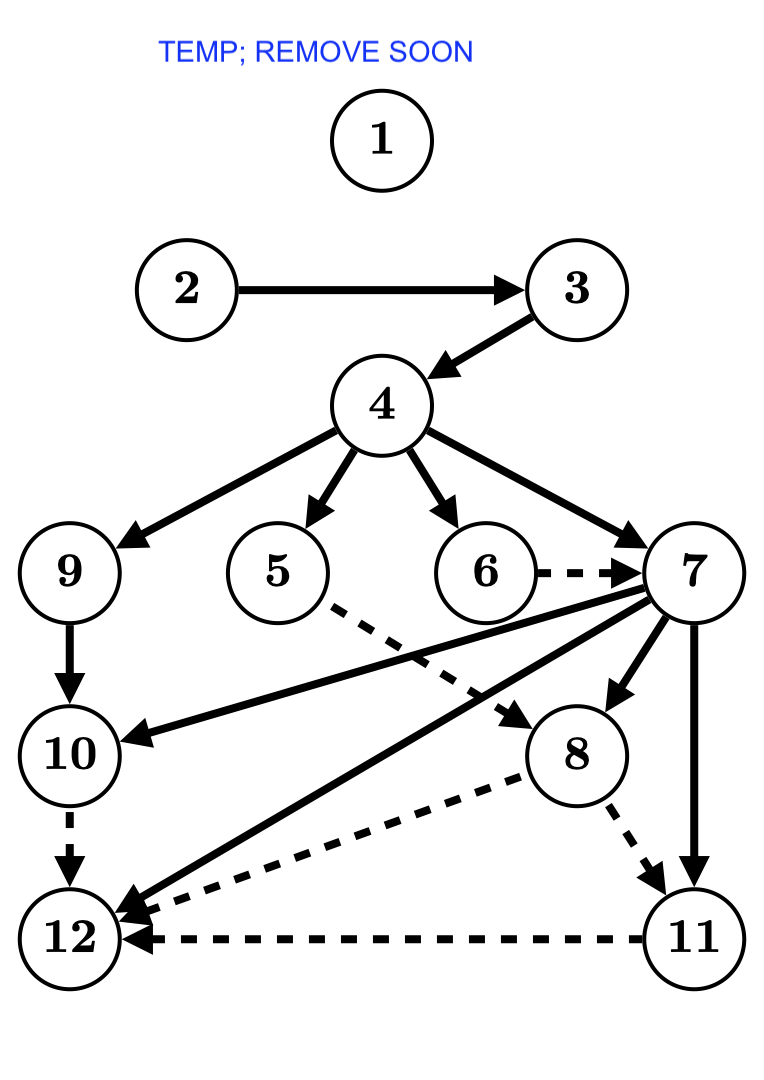
\includegraphics[width=\linewidth]{Interdependence.png}
    
    \newpage

    \textbf{Notes}:
    \interdependencenotes

    \mainmatter  % Now use arabic numerals for page numbers
}

%============= Index Pages ===============
\usepackage[
    totoc,
    columnsep=20pt,
    hangindent=8pt,
    subindent=20pt,
    subsubindent=30pt
]{idxlayout}

\makeindex[options= -s ../index-style.ist]

%======= Bibliography Formatting =========
% These two lines are here to ensure that URLs do not exceed the page by too much
\setcounter{biburllcpenalty}{7000}
\setcounter{biburlucpenalty}{8000}

\usepackage{xr}

%=========== Global Variables ============
\newcommand{\version}{0.1}
\newcommand{\volumenumber}{3}
\newcommand{\volumename}{Fields}
\newcommand{\volumeimage}{cover/Regular Heptagon.png}

%============= Formatting ================
\linespread{1.05}

%============== Resources ================
\externaldocument{../Volume 0/Volume0}

%========= Front Matter Pages ============
% Quote page
\newcommand{\quotepagetext}{
    I became convinced that studying the algebraic relationship of numbers is most conveniently based on a concept that is directly connected with the simplest arithmetic properties. I had originally used the term ``rational domain'', which I later changed to ``field''.
}
\newcommand{\quotepageattribution}{Richard Dedekind, 1871}
\newcommand{\quotepagecitation}{\cite[p.~66]{kleiner_2007}}

% Preface
\newcommand{\prefacevolumetext}{
    We cover field theory essentials in Volume III. %TODO: Add
}
\newcommand{\prefacevolumedate}{}  %TODO: Add

% Suggestions of use
\newcommand{\interdependencenotes}{
    \begin{itemize}
        \item Number 1
        \item number 2
        \item 3
    \end{itemize}
}

%=========================================
\begin{document}
\frontmatterpages  % Use lowercase roman numerals for page numbers

%=========================================
\chapter{Introduction to Fields}

%=========================================
\appendix
\section{Sets}
\begin{questions}
    \item \begin{partquestions}{\alph*}
        \item True, as both 1 and 2 appear in the set $\{1, 2, 3, 4\}$.
        \item False, 3 does not appear in $\{1, 2, 4\}$.
        \item True. Any set is a subset of itself, including the empty set.
        \item False, the set $S$ does not contain any element that is not in $S$. That is, $S \subseteq S$ but not $S \subset S$.
        \item True. $S$ is indeed an element of $\{S, \emptyset\}$.
        \item True. The set containing S is not an element of $\{S, \emptyset\}$.
        \item False, the set $S$ is not a subset of the set $\{S, \emptyset\}$.
        \item True. The set containing $S$ is a subset of the set containing $S$ and the empty set.
    \end{partquestions}
    
    \item \begin{partquestions}{\alph*}
        \item True.
        \item False, $S \cup U = \{1, 2, 3, 4, (2, 2), (3, 3), (5, 5)\}$.
        \item True.
        \item True.
        \item True.
        \item False, $S \setminus \{1, 4\} = \{2, 3\}$, not $T = \{2, 3, 5\}$.
        \item True.
        \item True. $(S \cup T)^2 = \{(1,1), (2,2), (3,3), (4,4), (5,5)\}$, so
        \[
            U = \{(2,2), (3,3), (5,5)\} \subset (S \cup T)^2.
        \]
    \end{partquestions}

    \item We note $S$ are all the non-positive rational numbers, and $T = \{-2, 0, 2, \dots, 8, 10\}$. Hence $S \cap T$ has only two elements, namely $-2$ and $0$.
\end{questions}

\section{Mathematical Logic}
\begin{questions}
    \item We work from the inner-most bracket outwards. We note $p$ is true, $q$ is false, and $r$ is true.
    \begin{itemize}
        \item $p \lor q$ is ``1 is a positive number \textbf{or} $-1 > 0$'', which is true since $p$ is true.
        \item $(p \lor q) \land r$ is ``(1 is a positive number or $-1 > 0$) \textbf{and} 1 is an odd number'', which is true since $p \lor q$ is true and 1 is, indeed, an odd number.
        \item $\lnot((p \lor q) \land r)$ is false, since $(p \lor q) \land r$ is true.
    \end{itemize}
    Hence the statement ``$\lnot((p \lor q) \land r)$ is false'' is a true statement.

    \item The truth table for $p \land \lnot q$ is given below.
    \begin{table}[H]
        \centering
        \begin{tabular}{|l|l||l|}
            \hline
            $\boldsymbol{p}$ & $\boldsymbol{q}$ & $\boldsymbol{p\land \lnot q}$ \\ \hline
            F   & F   & F                  \\ \hline
            F   & T   & F                  \\ \hline
            T   & F   & T                  \\ \hline
            T   & T   & F                  \\ \hline
        \end{tabular}
    \end{table}

    We will see that, in fact, this is the negation of $p \implies q$ later.

    \item \begin{partquestions}{\roman*}
        \item $r$: $n$ is a multiple of 5 if and only if the last digit of $n$ is 0 or 5.
        \item If $n$ is a multiple of 5, then its last digit necessarily has to be 5 or 0, hence $p \implies q$. If the last digit is 5 or 0, then the number $n$ is a multiple of 5, hence $q \implies p$. Therefore $p \iff q$.
    \end{partquestions}

    \item For brevity, let $r = p \implies \lnot q$ and $s = \lnot q \implies p$. So we want to show that $(\lnot p \iff q) \equiv r \land s$.
    \begin{table}[H]
        \centering
        \begin{tabular}{|l|l||l|l|l|l||l|l|}
            \hline
            $\boldsymbol{p}$ & $\boldsymbol{q}$ & $\boldsymbol{\lnot p}$ & $\boldsymbol{\lnot q}$ & $\boldsymbol{r}$ & $\boldsymbol{s}$ & $\boldsymbol{r \land s}$ & $\boldsymbol{\lnot p \iff q}$ \\ \hline
            F   & F   & T         & T         & T   & F   & F           & F                  \\ \hline
            F   & T   & T         & F         & T   & T   & T           & T                  \\ \hline
            T   & F   & F         & T         & T   & T   & T           & T                  \\ \hline
            T   & T   & F         & F         & F   & T   & F           & F                  \\ \hline
        \end{tabular}
    \end{table}

    From inspection, the truth tables of $\lnot p \iff q$ and $r \land s$ are the same, proving our required result.

    \item We work slowly.
    \begin{align*}
        &((p \lor \lnot q) \land \lnot r) \lor ((p \lor \lnot q) \land (p \lor r) \land (p \lor \lnot r))\\
        &\equiv ((p \lor \lnot q) \land \lnot r) \lor ((p \lor \lnot q) \land ((p \lor r) \land (p \lor \lnot r))) & (\text{Associativity})\\
        &\equiv (p \lor \lnot q) \land (\lnot r \lor ((p \lor r) \land (p \lor \lnot r))) & (\text{Distributivity})\\
        &\equiv (p \lor \lnot q) \land (\lnot r \lor (p \lor (r \land \lnot r))) & (\text{Distributivity})\\
        &\equiv (p \lor \lnot q) \land (\lnot r \lor (p \lor \textbf{false}))\\
        &\equiv (p \lor \lnot q) \land (\lnot r \lor p)\\
        &\equiv (p \lor \lnot q) \land (p \lor \lnot r) & (\text{Commutativity})\\
        &\equiv p \lor (\lnot q \land \lnot r) & (\text{Distributivity})\\
        &\equiv p \lor \lnot(q \lor r) & (\text{De Morgan's Law})
    \end{align*}

    \item $\left((n \in \mathbb{Z}) \land (n > 2)\right) \implies \left(\exists a, b \in \mathbb{Z} \text{ s.t. } a^3 + b^4 = n^5\right)$

    \item \begin{partquestions}{\roman*}
        \item Let
        \begin{align*}
            P(x):&\ (x \in \mathbb{R}) \land (x \neq 0)\\
            Q(x):&\ \exists y \in \mathbb{R} \text{ s.t. } xy = 1
        \end{align*}
        then the given statement is $\forall x, (P(x) \implies Q(x))$ as required.

        \item $\exists x \text{ s.t. } (x \in \mathbb{R}) \land (x \neq 0) \land (\forall y \in \mathbb{R}, xy \neq 1)$
    \end{partquestions}
\end{questions}

\section{Proof Writing}
\begin{questions}
    \item \begin{proof}
        Suppose $0 < x < 1$. Then $-1 < -x < 0$, meaning $0 < 1 - x < 1$. Therefore $x > 0$ and $1-x > 0$, so their product $x(1-x) > 0$.
    \end{proof}

    \item \begin{proof}
        Suppose that $m$ and $n$ have the same parity. We split into two cases.
        \begin{itemize}
            \item If both $m$ and $n$ are even, then we may write $m = 2a$ and $n = 2b$ where $a$ and $b$ are integers. Hence
            \begin{align*}
                m + n &= (2a) + (2b) \\
                &= 2(a+b)
            \end{align*}
            which clearly means that $m + n$ is even.
            \item If both $m$ and $n$ are odd, then we may write $m = 2a + 1$ and $n = 2b + 1$ where $a$ and $b$ are integers. Hence
            \begin{align*}
                m + n &= (2a + 1) + (2b + 1)\\
                &= 2a + 2b + 2\\
                &= 2(a + b + 1)
            \end{align*}
            which clearly means that $m+n$ is even.
        \end{itemize}
    Hence, in both cases, $m + n$ is even.
    \end{proof}

    \item We consider a proof by contrapositive; the statement that we want to prove is ''if \textbf{not} ($a$ is even or $b$ is odd) then $a(b^2+5)$ is \textbf{not} even''. That is, ''if $a$ is \textbf{not} even \textbf{and} $b$ is \textbf{not} odd then $a(b^2+5)$ is \textbf{not} even'', meaning ''if $a$ is odd and $b$ is even then $a(b^2+5)$ is odd''.

    \begin{proof}
        Suppose that $a$ is odd and $b$ is even. Then we may write $a = 2m + 1$ and $b = 2n$ where $m$ and $n$ are integers. Hence
        \begin{align*}
            a(b^2+5) &= (2m+1)\left((2n)^2 + 5\right)\\
            &= (2m+1)(4n^2 + 5)\\
            &= 8mn^2 + 10m + 4n^2 + 5\\
            &= 8mn^2 + 10m + 4n^2 + 4 + 1\\
            &= 2(4mn^2 + 5m + 2n^2 + 2) + 1
        \end{align*}
    which clearly means that $a(b^2+5)$ is odd.
    \end{proof}

    \item \begin{proof}
        By way of contradiction assume there exist integers $a$ and $b$ such that $2a + 4b = 1$. Then dividing both sides by 2 leads to $a + 2b = \frac12$. Note the left hand side is clearly an integer, while the right hand side is not an integer, a contradiction.
    \end{proof}

    \item \begin{proof}
        By way of contradiction assume that $a$ and $b$ are positive real numbers, and $\frac{a+b}{2} < \sqrt{ab}$. This means $a+b<2\sqrt ab$. Squaring both sides yields $(a+b)^2 < 4ab$. Note
        \[
            (a+b)^2 = a^2 + 2ab + b^2 < 4ab
        \]
        which implies $a^2 + b^2 < 2ab$, leading to $a^2 - 2ab + b^2 < 0$. However $a^2 - 2ab + b^2 = (a-b)^2 \geq 0$ for all positive real numbers $a$ and $b$. Hence we have $(a-b)^2 < 0$ and $(a-b)^2 \geq 0$, a contradiction.
    \end{proof}

    \item We note that a positive odd number is of the form $2n - 1$ where $n$ is a positive integer.

    \begin{proof}
        Set $a = 2n - 1$; we induct on $n$.

        When $n = 1$, we have $a^2 - 1 = (2(1) - 1)^2 - 1 = 1 - 1 = 0$ which is clearly a multiple of 8.

        Assume that the statement holds for some positive integer $k$, i.e. $(2k-1)^2 - 1 = 8m$ for some integer $m$. We show that the statement holds for $k + 1$.

        We note that $(2k-1)^2 - 1 = 4k^2 - 4k$. Observe
        \begin{align*}
            (2(k+1)-1)^2 - 1 &= (2k+1)^2 - 1\\
            &= 4k^2 + 4k + 1 - 1\\
            &= (4k^2 - 4k) + 8k\\
            &= 8m + 8k & (\text{by hypothesis})\\
            &= 8(m+k)
        \end{align*}
        which means that $(2(k+1)-1)^2 - 1$ is a multiple of 8, proving that the statement holds for $k+1$. By mathematical induction, $a^2 - 1$ is a multiple of 8 for all positive odd integers $a$.
    \end{proof}

    \item \begin{proof}
        We use strong induction on $n$.

        When $n = 2$ the statement is true since 2 is prime.

        Now assume that for some positive integer $k \geq 2$, every integer $m$ satisfying $2 \leq m \leq k$ results in the statement being true, i.e. $m$ is either prime or can be expressed as a product of primes. We are to show that the statement is true for $k + 1$, i.e. $k+1$ is prime or can be expressed as a product of primes.

        Now if $k + 1$ is prime we are done. Otherwise $k + 1$ is composite, meaning that $k + 1 = ab$ for some integers $2 \leq a,b \leq k$. Applying the induction hypothesis on $a$ and $b$ means that $a$ and $b$ are primes or product of primes. Thus $k + 1$ is a product of primes.

        Therefore by mathematical induction, every integer $n \geq 2$ is either prime or can be expressed as a product of primes.
    \end{proof}

    \item \begin{proof}
        We prove the forward direction using direct proof. Assume $n$ is one more than a multiple of 5. Then we may write $n = 5a + 1$ where $a$ is an integer. Note $5a + 1 = 5a + (5 - 4) = (5a + 5) - 4 = 5(a+1) - 4$. Setting $k = a+1$ yields required result.

        We now prove the reverse direction, using direct proof as well. Assume $n = 5k - 4$. Observe $5k - 4 = 5k - 5 + 1 = 5(k-1) + 1$, meaning $n$ is one more than a multiple of 5.
    \end{proof}

    \item \begin{proof}
        The number 7 satisfies this as $7 = 2^3 - 1$ and $7 = 3^2 - 2$.
    \end{proof}

    \item \begin{partquestions}{\roman*}
        \item We use a proof by contradiction to prove this claim.

        \begin{proof}
            Seeking a contradiction, assume $y$ is rational. Write $y = \frac pq$ where $p$ and $q$ are integers. Note $2^y = 2^{\frac pq}$ and $2^y = 2^{2\log_2{3}} = 9$. Hence $2^{\frac pq} = 9$ meaning $2^p = 9^q$. However $2^p$ is always even and $9^q$ is always odd, a contradiction.
        \end{proof}

        \item \begin{proof}
            Note
            \[
                x^y = (\sqrt2)^{2\log_2{3}} = \left(\sqrt{2}^2\right)^{\log_2{3}} = 2^{\log_2{3}} = 3
            \]
            which is rational.
        \end{proof}
    \end{partquestions}
\end{questions}

\section{Algebra}
\begin{questions}
    \item \begin{partquestions}{\alph*}
        \item $\displaystyle \sum_{i=3}^{5}(7ix+11) = (7\times3x + 11) + (7\times4x + 11) + (7\times5x + 11) = 84x + 33$.
        \item $\displaystyle \sum_{x=3}^{5}(7ix+11) = (7i\times3 + 11) + (7i\times4 + 11) + (7i\times5 + 11) = 84i + 33$.
        \item Since the upper bound is smaller than the lower bound, the sum evaluates to 0.
        \item $\displaystyle \sum_{i=4}^{8}ijk = 4jk + 5jk + 6jk + 7jk + 8jk = 30jk$.
        \item $\displaystyle \sum_{j=4}^{8}ijk = 4ik + 5ik + 6ik + 7ik + 8ik = 30ik$.
        \item $\displaystyle \sum_{n=4}^{8}ijk = ijk + ijk + ijk + ijk + ijk = 5ijk$.
        \item $\displaystyle \sum_{i=3}^{7}13 = 13 + 13 + 13 + 13 + 13 = 65$.
        \item $\displaystyle \sum_{i=1}^{3}i^2 + \sum_{j=4}^{6}j^2 = (1^2 + 2^2 + 3^2) + (4^2 + 5^2 + 6^2) = 91$.
        \item $\displaystyle \sum_{i=1}^{3}\left(\sum_{j=5}^{7}(i+j)\right) = \sum_{i=1}^{3}\left((i+5) + (i+6) + (i+7)\right) = \sum_{i=1}^{3}\left(3i+18\right) = (3\times1 + 18) + (3\times2 + 18) + (3\times3 + 18) = 72$.
    \end{partquestions}

    \item Note $\displaystyle \sum_{i=2}^5a_{i-1} = \sum_{i=1}^4a_i = 10$. Also
    \begin{align*}
        200 = \sum_{i=1}^5(a_i+2)^2 &= \sum_{i=1}^5(a_i^2 + 4a_i + 4)\\
        &= \sum_{i=1}^5a_i^2 + 4\sum_{i=1}^5a_i + \sum_{i=1}^54\\
        &= \sum_{i=1}^5a_i^2 + 4\left(\sum_{i=1}^4a_i + \sum_{i=5}^5a_i\right) + \sum_{i=1}^54\\
        &= 100 + 4\left(10 + a_5\right) + 20\\
        &= 160 + 4a_5
    \end{align*}
    which therefore means $a_5 = 10$.

    \item Rearrange $x^2 + 15 < 8|x|$ to become $x^2 - 8|x| + 15 < 0$, meaning $|x|^2 - 8|x| + 15 < 0$. Note $|x|^2 - 8|x| + 15 = (|x|-3)(|x|-5)$, so we are solving $(|x|-3)(|x|-5)<0$. Therefore $3 < |x| < 5$.
    \begin{itemize}
        \item If $|x| = -x$ (i.e., $x$ is negative), then $3 < -x < 5$, which means $-5 < x < -3$.
        \item If $|x| = x$ (i.e. $x$ is non-negative), then $3 < x < 5$.
    \end{itemize}
    Hence $-5 < x < -3$ or $3 < x < 5$.

    \item The relevant term is
    \[
        {9 \choose 7}(7x)^7(-3)^{9-7} = -266827932x^6
    \]
    so its coefficient is -266827932.
\end{questions}

\section{Functions / Maps}
\begin{questions}
    \item \begin{partquestions}{\roman*}
        \item $f: \{1, 2, 3\} \to \{1, 4, 9, 16, 25\}, x \mapsto x^2$. (Or just $x \mapsto x^2$)
        \item Domain is $\{1, 2, 3\}$, codomain is $\{1, 4, 9, 16, 25\}$, range is $\{1, 4, 9\}$.
        \item The image of 2 under $f$ is $2^2 = 4$.
        \item No. The element 3 would map to 27, which is not in the codomain.
    \end{partquestions}
    
    \item It is not well-defined. Note $\frac 12 = \frac 24$, but $f(\frac12) = 1 + 2 = 3$ and $f(\frac24) = 2 + 4 = 6$.
    
    \item $fg(x) = \left(\frac1{x^2+1}\right)^2 - \frac1{x^2+1} + 1$.
    
    \item We prove the requirements of a bijection one by one.
    \begin{itemize}
        \item \textbf{Injective}: Suppose $x_1, x_2 \in \mathbb{N}$ such that $f(x_1) = f(x_2)$. We split into three cases.
        \begin{itemize}
            \item The first case is if $f(x_1) = f(x_2) = 0$. In this case, one sees clearly that $x_1 = x_2 = 1$.
            \item The second case is if $f(x_1) = f(x_2) > 0$. Now since $x \neq 1$ (as this case leads to $f(x_1) = 0$), the `valid' odd numbers are at least 3. Therefore, $\frac{1-x}{2} \leq \frac{1-3}{2} = -1 < 0$, so $x_1$ and $x_2$ cannot be odd. Hence, $x_1$ and $x_2$ are even, meaning $\frac{x_1}{2} = \frac{x_2}{2}$ which quickly implies $x_1 = x_2$.
            \item The third case is if $f(x_1) = f(x_2) < 0$. As argued above, this means that $x_1$ and $x_2$ must be odd numbers of at least 3. Hence, $\frac{1-x_1}{2} = \frac{1-x_2}{2}$ which quickly implies $x_1 = x_2$.
        \end{itemize}
        Thus, in all three cases, $f(x_1) = f(x_2)$ implies $x_1 = x_2$, meaning $f$ is injective.
        \item \textbf{Surjective}: Suppose $y \in \mathbb{Z}$. We split into three cases again.
        \begin{itemize}
            \item If $y = 0$, then setting $x = 1$ satisfies $f(x) = y$.
            \item Now suppose $y > 0$. We note $2y \in S$, and clearly $2y$ is an even integer. So setting $x = 2y$ satisfies $f(x) = \frac{2y}{y} = y$.
            \item Suppose $y < 0$. Note $-2y > 0$, and $1 - 2y > 0 \in S$. Furthermore $1 - 2y$ is clearly an odd integer. Hence setting $x = 1 - 2y$ satisfies $f(x) = \frac{1-(1-2y)}{2} = y$.
        \end{itemize}
        Therefore for every $y \in \mathbb{Z}$, there exists a pre-image $x \in \mathbb{N}$ such that $f(x) = y$. Hence $f$ is surjective.
    \end{itemize}
    Therefore, as $f$ is both injective and surjective, $f$ is bijective. Hence, $|\mathbb{N}| = |\mathbb{Z}|$.
\end{questions}

\section{Elementary Number Theory}
\begin{questions}
    \item $44100 = 2^2 \times 3^2 \times 5^2 \times 7^2$.
    \item $-210 = 11 - 13 \times 17$, so $a = 11$ and $b = 17$.
    \item $\gcd(-112, -35) = 7$ since $-112 = -16 \times 7$ and $-35 = -5 \times 7$, with 7 being the largest integer that achieves this.
    \item $\lcm(-112, -35) = 560$ since $560 = -5 \times -112$ and $-35 = -16 \times -35$, with 560 being the smallest \textit{positive} integer that achieves this.
    \item \begin{partquestions}{\roman*}
        \item $\gcd(42, 70) = 14$ since $42 = 3 \times 14$ and $70 = 5 \times 14$, and 14 is the largest integer achieving this.
        \item $\lcm(42, 70) = \frac{42 \times 70}{\gcd(m, n)} = \frac{2940}{14} = 210$ by \myref{prop-product-of-gcd-and-lcm}.
        \item Note that $x = 2$ and $y = -1$ works as $42 \times 2 + 70 \times (-1) = 84 - 70 = 14$.
    \end{partquestions}
\end{questions}

\section{Modular Arithmetic}
\begin{questions}
    \item \begin{partquestions}{\alph*}
        \item $17 \mod 5 = 2$ since $17 = 3 \times 5 + 2$ by the division algorithm.
        \item As $19 = 3 \times 5 + 4$, thus $19 \equiv 4 \pmod 5$. Hence $x = 4$.
        \item $A \mod n = 5 \mod 3 = 2$.
    \end{partquestions}
    
    \item $-n = (-1) \times 2n + n$, which means that $-n \equiv n \pmod{2n}$.
    
    \item Finding the last two digits of a number is the same as finding the remainder of that number when divided by 100. We note $778899 \equiv 99 \pmod{100}$, so $778899^{112233} \equiv 99^{112233} \pmod{100}$. Furthermore, $99 \equiv -1 \pmod{100}$, so $99^{112233}\equiv (-1)^{112233} \equiv -1 \equiv 99 \pmod{100}$. Hence the last two digits of $778899^{112233}$ are both 9.
    
    \item Note $123 \equiv 3 \pmod 5$. One can easily find by trial and error that 2 is the multiplicative inverse of 3, since $3 \times 2 = 6 \equiv 1 \pmod 5$. Hence the multiplicative inverse of 123 is 2 modulo 5.
\end{questions}


\chapter{Problem Solutions}
\section{Introduction to Groups}
\begin{questions}
    \item \begin{partquestions}{\alph*}
        \item This is a group. Addition is clearly closed and associative. The identity is 0. The inverse of any element $x$ is $-x$.
        \item This is not a group. Inverses do not exist. For example, the element $2$ does not have an inverse under multiplication.
        \item This is a group. Multiplication is clearly closed and associative. The identity is $1$. The inverse of any element $x$ is $\frac1x$.
        \item This is a group. Multiplication is clearly closed and associative. The identity is $0$ and the inverse is $0$.
        \item This is not a group. Addition is not closed: $1 + 1 = 2$ which is not in the group.
        \item This is a group. Multiplication is clearly closed and associative. The identity is $1$ and the inverse is $1$.
    \end{partquestions}

    \item We show that the trivial group is indeed a group by showing that the four group axioms hold.
    \begin{itemize}
        \item \textbf{Closure}: The only element in the underlying set is $e$, and $e \ast e = e \in \{e\}$. Thus the structure is closed under $\ast$.
        \item \textbf{Associativity}: Clearly $e \ast (e \ast e) = e \ast e = e$ and $(e \ast e) \ast e = e \ast e = e$ which means that $\ast$ is associative.
        \item \textbf{Identity}: The identity is clearly $e$.
        \item \textbf{Inverse}: The only element is $e$, and because $e \ast e = e$ hence $e$ is its own inverse.
    \end{itemize}
    Therefore $(\{e,\}, \ast)$ is a group.
\end{questions}

\section{Basics of Groups}
\begin{questions}
    \item The group table of $D_4$ is given below.
    \begin{table}[h]
        \centering
        \begin{tabular}{|l|l|l|l|l|l|l|l|l|}
        \hline
        $\ast$ & $e$    & $r$    & $r^2$  & $r^3$  & $s$    & $rs$   & $r^2s$ & $r^3s$ \\ \hline
        $e$    & $e$    & $r$    & $r^2$  & $r^3$  & $s$    & $rs$   & $r^2s$ & $r^3s$ \\ \hline
        $r$    & $r$    & $r^2$  & $r^3$  & $e$    & $rs$   & $r^2s$ & $r^3s$ & $s$    \\ \hline
        $r^2$  & $r^2$  & $r^3$  & $e$    & $r$    & $r^2s$ & $r^3s$ & $s$    & $rs$   \\ \hline
        $r^3$  & $r^3$  & $e$    & $r$    & $r^2$  & $r^3s$ & $s$    & $rs$   & $r^2s$ \\ \hline
        $s$    & $s$    & $r^3s$ & $r^2s$ & $rs$   & $e$    & $r^3$  & $r^2$  & $r$    \\ \hline
        $rs$   & $rs$   & $s$    & $r^3s$ & $r^2s$ & $r$    & $e$    & $r^3$  & $r^2$  \\ \hline
        $r^2s$ & $r^2s$ & $rs$   & $s$    & $r^3s$ & $r^2$  & $r$    & $e$    & $r^3$  \\ \hline
        $r^3s$ & $r^3s$ & $r^2s$ & $rs$   & $s$    & $r^3$  & $r^2$  & $r$    & $e$    \\ \hline
        \end{tabular}
    \end{table}
    \begin{partquestions}{\alph*}
        \item $D_4$ is not abelian because $rs \neq sr = r^3s$.
        \item We simplify $r^3srsr^3sr^3sr^2$.
        \begin{align*}
            r^3 sr sr^3 sr^3 sr^2 &= r^3srs(r^3s)(r^3s)r^2\\
            &= r^3 srs(e)r^2\\
            &= r^3 sr sr^2\\
            &= r^2(rs rs)r^2\\
            &= r^2(e)r^2\\
            &= r^4\\
            &= e
        \end{align*}
    \end{partquestions}

    \item If every element in $G$ is its own inverse, then for every element $g$ in $G$, $g^{-1} = g$. Consider $(gh)^{-1}$ where $g$ and $h$ are elements in $g$. On one hand, by Shoes and Socks, $(gh)^{-1} = h^{-1}g^{-1} = hg$ since each element is its own inverse. On the other hand, since $gh$ is an element in $G$, thus $(gh)^{-1} = gh$. Thus $gh = hg$ which means $G$ is abelian.
    
    \item Recall that $n = |x|$ is the smallest positive integer that satisfies $x^n = e$.
    
    We prove the forward direction first. Suppose $m$ is a multiple of $n$, say $m = qn$ for some integer $q$. Then
    \[
        x^m = x^{qn} = \left(x^n\right)^q = e^q = e    
    \]
    which means $x^m = e$.
    
    We now prove the reverse direction. Suppose $x^m = e$. Using Euclid's division lemma (\myref{lemma-euclid-division}), we write $m = qn + r$ where $q$ and $r$ are integers with $0 \leq r < n$. Hence
    \[
        x^m = x^{qn + r} = x^{qn}x^r = \left(x^n\right)^qx^r = e^qx^r = x^r.
    \]
    Note that for all integers $k$ where $1 \leq k < n$, we have $x^k \neq e$ since $n$ is the smallest positive integer such that $x^n = e$. Hence, if $x^r = e$, we conclude $r = 0$. Therefore $m = qn$, meaning $m$ is a multiple of $n$.

    \item \begin{partquestions}{\alph*}
        \item Note that $(gh)^2 = ghgh$. Given that $(gh)^2 = g^2h^2 = gghh$. By cancellation law, $hg = gh$ which means $G$ is abelian.
        \item Suppose $G$ is abelian. Clearly $(gh)^1 = gh$. Suppose $(gh)^{k} = g^kh^k$ for some positive integer $k$. Then
        \begin{align*}
            (gh)^{k+1} &= (gh)(gh)^k\\
            &= (gh)(g^kh^k) & (\text{by assumption})\\
            &= ghg^kh^k\\
            &= g(hg^k)h^k\\
            &= g(g^kh)h^k & (\text{since } G \text{ is abelian})\\
            &= gg^khh^k\\
            &= g^{k+1}h^{k+1}
        \end{align*}
        so $(gh)^{k+1} = g^{k+1}h^{k+1}$ assuming $(gh)^k = g^kh^k$. Thus the claim is proven by mathematical induction.
    \end{partquestions}

    \item Note that $|1| = n$ since $1^2 = 1 \oplus_n 1 = 2$, $1^3 = 1 \oplus_n 1 \oplus_n 1 = 3$, $1^4 = 4$, ..., $1^{n-1} = n-1$ and $1^n = 0$ which is the identity. Since the group $(\mathbb{Z}_n, \oplus_n)$ has an element with the same order as the group, it is thus cyclic with order $n$ and generator 1.

    \item We show that $(A, \circ)$ is a group.
    \begin{itemize}
            \item \textbf{Closure}: Function composition is closed by definition.
            \item \textbf{Associativity}: Function composition is associative.
            \item \textbf{Identity}: By performing brute-force computation, we find that $T^6(x, y) = (x, y)$. Hence $T^6$ is the identity of $A$.
            \item \textbf{Inverse}: If $r = 6$ then $T^r$ is its own inverse. Otherwise, $T^{6-r}$ is the inverse of $T^r$.
    \end{itemize}
    Thus, $(A, \circ)$ is a group, with order 6.
\end{questions}

\section{Subgroups}
\begin{questions}
    \item We note that $G$ contains $\{e, r, r^2, r^3, s, rs, r^2s, r^3s\}$.
    \begin{partquestions}{\alph*}
        \item Yes, this is the trivial subgroup.
        \item No, it is not closed. ($rs$ can be generated by $r \ast s$ but is not in the set)
        \item No, the identity $e$ is missing.
        \item Yes, $\{r, r^3, r^4, r^6\} = \{r, r^3, e, r^2\} = \langle r \rangle$ which is a cyclic subgroup of $G$.
    \end{partquestions}

    \item \begin{partquestions}{\alph*}
        \item Clearly $K$ is a subset of $G$. Note $e \in K$ since $e^2 = e \in H$, so $K$ is non-empty.
        
        Let $x, y \in K$, so $x^2 \in H$ and $y^2 \in H$. We note $y^{-1} \in K$ since $(y^{-1})^2 = (y^2)^{-1} \in H$. Therefore $(xy^{-1})^2 = xy^{-1}xy^{-1} \in H$, so $xy^{-1} \in K$. Hence $K \leq G$ by subgroup test (\myref{thrm-subgroup-test}).

        \item We show that $H \subseteq K$. Note that for any $h \in H$ we have $h^2 \in H$ (since $H$ is a (sub)group and so it is closed). Thus $h \in K$. This shows that $H \subseteq K$. Now because $H \subseteq K$ and $H$ is a (sub)group, thus $H \leq K$ by definition of subgroup.
    \end{partquestions}

    \item \begin{partquestions}{\alph*}
        \item We have proved that $\Z{G} \leq G$ so we only prove normality. Let $g$ and $z$ be arbitrary elements from $G$ and $\mathrm{Z}(G)$ respectively. Then
        \begin{align*}
            gzg^{-1} &= g(zg^{-1})\\
            &= g(g^{-1}z) & (\text{since }z \in \mathrm{Z}(G))\\
            &= (gg^{-1})z \\
            &= z\\
            &\in \mathrm{Z}(G)
        \end{align*}
        which proves that $\mathrm{Z}(G) \unlhd G$.

        \item We first work in the forward direction by assuming $G = \Z{G}$. Then for all $z \in \Z{G} = G$ we have $gz = zg$ for any $g \in G$ by definition, which means that $G$ is abelian.

        We now work in the reverse direction by assuming that $G$ is abelian. Note $\mathrm{Z}(G) = \{z \in G \vert gz = zg \text{ for all } g \in G\}$. But since $G$ is abelian, $gh = hg$ for all $g$ and $h$ in $G$. Thus every element in $G$ satisfies the condition to be in the center of $G$, meaning $\mathrm{Z}(G) = G$.

        \item We note that $D_4 = \{e, r, r^2, r^3, s, rs, r^2s, r^3s\}$. Since $\mathrm{Z}(D_4)$ is a subgroup of $D_4$ it has a maximum order of 2, by Lagrange's theorem (\myref{thrm-lagrange}) and the note given. Since 2 is prime the subgroups must be cyclic. Thus the non-trivial proper subgroups of $D_4$ are $\{e, r^2\}$ and $\{e, s\}$ (since $|r^2| = |s| = 2$). Now like how we proved that $\langle s \rangle = \{e, s\}$ is not a normal subgroup in $D_3$ in \myref{example-normal-subgroups-of-d3}, $\{e, s\}$ is not a normal subgroup of $D_4$. One verifies easily that $\{e, r^2\} = \langle r^2 \rangle$ is a normal subgroup of $D_4$. Thus $\mathrm{Z}(D_4) = \langle r^2 \rangle$ since $\mathrm{Z}(D_4)$ must be a normal subgroup of $D_4$ with order not exceeding 2.
    \end{partquestions}

    \item \begin{partquestions}{\alph*}
        \item We will prove this statement.

        Clearly since $H \subseteq G$ and $K \subseteq G$ (as both are subgroups), thus $H \cap K \subseteq G$. Also $e \in H \cap K$ since $e \in H$ and $e \in K$ as both are subgroups of $G$. Therefore $H \cap K$ is non-empty.

        Let $x$ and $y$ be in $H \cap K$, meaning that $x, y \in H$ and $x, y \in K$. Thus $xy^{-1} \in H$ and $xy^{-1} \in K$ as both are subgroups of $G$. Hence $xy^{-1} \in H \cap K$.
        
        Therefore $H \cap K \leq G$ by the subgroup test (\myref{thrm-subgroup-test}).

        \item We will prove this statement. One sees that $H \cap K \subseteq H$. Since $H \cap K \leq G$, it is thus a group. Hence $H \cap K \leq H$ by definition of a subgroup.

        \item We will disprove this statement. Consider
        \begin{align*}
            &G = \mathbb{Z}_6 \text{ under }\oplus_6,\\
            &H = \{0, 2, 4\},\text{ and}\\
            &K = \{0, 3\}.
        \end{align*}
        Clearly $H \leq G$ and $K \leq G$. Note $H \cup K = \{0, 2, 3, 4\}$. But $H \cup K$ is not closed since $2 \oplus_6 3 = 5 \not \in H \cup K$. Hence $H \cup K \not\leq G$.

        \item We will disprove this statement. Since $H \cup K$ is not closed it is not a group, meaning it cannot be a subgroup.
    \end{partquestions}

    \item By Lagrange's Theorem (\myref{thrm-lagrange}), the order of a subgroup must divide the order of the group. Since $H \leq G$ is proper, and since $1024 = 2^{10}$, the largest order that $H$ can be is $512$ with $[G:H] = 2$. An example is $G = \mathbb{Z}_{1024}$ and $H = \langle 2 \rangle$, since $|H| = |2| = 512$ as $2 \times 512 = 1024 \equiv 0 \pmod{1024}$.

    \item Let $|G| = 2n$. The identity is its own inverse, leaving an odd number of non-identity elements.
    
    Suppose $x$ is an element of $G$ with $|x| > 2$; we cannot have $x^{-1} = x$ (otherwise $x^2 = e$). Thus $x^{-1}$ and $x$ are distinct. Pair every one of these $x$'s with its inverse $x^{-1}$.

    Remember that there is an odd number of non-identity elements. Hence, there must be at least one element which has not been paired off with any of the others, which is therefore its own self inverse.

    Since this element is not the identity, thus it has to have order 2 (as $g^{-1} = g$ implies $g^2 = e$).

    \item Suppose $G = \langle g \rangle$ and $H \leq G$. Then any element in $H$ is of the form $g^a$ where $a$ is an integer. Suppose $m$ is the smallest positive integer $m$ such that $g^m \in H$. Suppose now $g^n \in H$ for some $n$. By Euclid's division lemma (\myref{lemma-euclid-division}), $n = mq + r$ where $q$ and $r$ are non-negative integers such that $0 \leq r < m$. Hence,
    \[
        g^n = g^{mq}g^r = (g^m)^q g^r.
    \]
    Now, $m$ is the smallest positive integer such that $g^m \in H$. This means that if $r \neq 0$, $g^r \not\in H$ as $0 \leq r < m$. Hence, $r = 0$, which means
    \[
        g^n = (g^m)^q.
    \]
    Thus, every element in the subgroup $H$ can be formed by applying $g^m$ a certain number of times, meaning $H$ is cyclic with generator $g^m$.

    \item \begin{partquestions}{\roman*}
        \item Let $xH$ be a coset in $G$. Since cosets partition $G$, either $xH = H$ or $xH = G \setminus H$ (since there are only two distinct cosets).
        \begin{itemize}
                \item If $xH = H$, then $xH = Hx$ by Element in Coset (\myref{corollary-equivalence-of-element-in-coset}).
                \item If $xH = G \setminus H$, then $xH \neq H$, meaning $Hx \neq H$ by contrapositive of Element in Coset. But if $Hx \neq H$, then $Hx = G \setminus H$ (since there are only two distinct cosets). So $xH = G \setminus H = Hx$.
        \end{itemize}
        Therefore $H$ is a normal subgroup of $G$, i.e. $H \lhd G$.

        \item Note that $G/H$ is a group since $H \lhd G$. Also since $[G:H] = 2$ thus $|G/H| = 2$.
        
        If $x \in G$ then $x^2H = (xH)^2 = H$ since the order of $G/H$ is 2, meaning that any non-identity element inside it (like $xH$) has an order of at most 2. Since $x^2H = H$, therefore $x^2 \in H$ by Element in Coset (\myref{corollary-equivalence-of-element-in-coset}).
        
        \item Suppose $x$ has odd order. Write $|x| = 2k - 1$ where $k$ is a positive integer. Hence $x^{2k-1} = e \in H$ since $H < G$. Therefore
        \[
            x = x^{2k} = \left(x^k\right)^2 \in H        
        \]
        which means $x \in H$.
    \end{partquestions}

    \item \begin{partquestions}{\alph*}
        \item Suppose we have an element $x \in H \cap K$, meaning that $x \in H$ and $x \in K$. By a corollary of Lagrange's Theorem (\myref{corollary-order-of-group-multiple-of-order-of-element}), the order of $x$ must divide the order of its group. Hence, $|x|$ divides $|H|$ and $|x|$ divides $|K|$ simultaneously, meaning that $|x| = \gcd(|H|, |K|)$. But the GCD of the orders of both subgroups is 1. Hence, $|x| = 1$, meaning the only element in the intersection $H \cap K$ is the identity $e$.
        
        \item Consider $hkh^{-1}k^{-1}$.
        \begin{itemize}
            \item On one hand, note that $hkh^{-1}k^{-1} = h(kh^{-1}k^{-1})$. Clearly $h \in H$ and $kh^{-1}k^{-1} \in H$ by normality of $H$. Therefore $hkh^{-1}k^{-1} \in H$.
            \item On another hand, $hkh^{-1}k^{-1} = (hkh^{-1})k^{-1}$. Note $hkh^{-1} \in K$ by normality of $K$ and $k^{-1} \in K$, so $hkh^{-1}k^{-1} \in K$.
        \end{itemize}
        Therefore $hkh^{-1}k^{-1} \in H \cap K$. But by \textbf{(a)}, the only element in $H \cap K$ is the identity. Thus, $hkh^{-1}k^{-1} = e$ which the result follows quickly.
    \end{partquestions}
    
    \item \begin{partquestions}{\alph*}
        \item $m = 6$.
        \item We first prove that all groups of order less than 6 are abelian, and then find a non-abelian group of order 6.

        We note that a group of order 1 is the trivial group which is abelian. The groups of order 2, 3, and 5 are groups of prime order, meaning that they are cyclic and hence abelian. We are left with a group of order 4.

        We note that the order of an element of a group of order 4 must divide 4 (\myref{corollary-order-of-group-multiple-of-order-of-element}). Hence the possible orders of an element in such a group is 1, 2, or 4. An element of order 1 is the identity. If an element with order 4 exists, then the group is cyclic and hence abelian. So we assume that all elements are either order 1 or order 2 (in fact, the orders must be 1, 2, 2, 2). This is precisely the group
        \[
            D_2 = \langle r, s \vert r^2 = s^2 = e, rs = sr\rangle
        \]
        which is abelian. Hence all groups of order 4 are abelian.

        We now show that a group of order 6 can be non-abelian. We note that the group
        \[
            D_3 =  \langle r, s \vert r^3 = s^2 = e, rs = sr^2\rangle
        \]
        has order 6 and because $rs = sr^2 \neq sr$, thus $D_3$ is non-abelian. Hence $m = 6$.

        \item For all even $n \geq 6$, the group $D_{\frac n2}$ has $n$ elements and $rs = sr^{\frac n2 - 1} \neq sr$, so $D_{\frac n2}$ is non-abelian.
    \end{partquestions}

    \item Suppose $G / \Z{G}$ is cyclic. Then by definition, $G / \Z{G} = \langle g\Z{G}\rangle$ for some $g \in G$, and any element in $G/\Z{G}$ is of the form $g^n\Z{G}$.

    Now take $x, y \in G$. By \myref{lemma-left-coset-partition}, left cosets partition the group, so we may assume $x \in g^m\Z{G}$ and $y \in g^n\Z{G}$, meaning $x = g^mz_1$ and $y = g^nz_2$ for some $z_1, z_2 \in \Z{G}$. We note
    \begin{align*}
        xy &= (g^mz_1)(g^nz_2)\\
        &= g^m(z_1g^n)z_2\\
        &= g^m(g^nz_1)z_2 & (\text{since }z_1 \in \Z{G})\\
        &= (g^mg^n)(z_1z_2)\\
        &= g^{m+n}z_1z_2\\
        &= g^{n+m}z_2z_1\\
        &= g^ng^mz_2z_1\\
        &= g^n(g^mz_2)z_1\\
        &= g^n(z_2g^m)z_1\\
        &= (g^nz_2)(g^mz_1)\\
        &= yx
    \end{align*}
    which means that $xy = yx$ for any $x, y \in G$. Hence $G$ is abelian.
\end{questions}

\section{Homomorphisms and Isomorphisms}
\begin{questions}
    \item We will prove that $f$ is a homomorphism, is injective, and is surjective.
    \begin{itemize}
        \item \textbf{Homomorphism}: Let $x, y \in G$. Then
        \begin{align*}
            f(xy) &= g(xy)g^{-1}\\
            &= (gxg^{-1})(gyg^{-1})\\
            &= f(x)f(y)
        \end{align*}
        which means that $f$ is a homomorphism.
        \item \textbf{Injective}: Let $x, y \in G$ be such that $f(x) = f(y)$. Then $gxg^{-1} = gyg^{-1}$. By cancellation law, $x = y$.
        \item \textbf{Surjective}: Suppose $y \in G$. Set $x = g^{-1}yg$. Since $G$ is closed, thus $x \in G$. Note $f(x) = g(g^{-1}yg)g^{-1} = y$. Hence $y$ has a pre-image of $x = g^{-1}yg$ in $G$.
    \end{itemize}
    Therefore $f$ is an isomorphism.

    \item Suppose on the contrary there exists an isomorphism $\phi: G \to H$. Since $\phi$ is an isomorphism, it is surjective. Hence, there must exists a rational number $r \in G$ such that $\phi(r) = 2$. As $r$ is rational, so is $\frac r2$.

    Now consider $\phi\left(\frac r2 + \frac r2\right)$. On one hand, $\phi\left(\frac r2 + \frac r2\right) = \phi(r) = 2$. On another hand, $\phi(\frac r2 + \frac r2) = \left(\phi\left(\frac r2\right)\right)^2$ as $\phi$ is a homomorphism. Therefore, $\left(\phi\left(\frac r2\right)\right)^2 = 2$ which quickly implies $\phi\left(\frac r2\right) = \sqrt 2$ since $\phi\left(\frac r2\right)$ must be positive. However, $\sqrt 2 \notin H$ while $\phi\left(\frac r2\right) \in H$, a contradiction.

    Hence, $G \not\cong H$.

    \item \begin{partquestions}{\alph*}
        \item Let $m, n \in \mathbb{Z}$. Then
        \[
            \phi(m + n) = 2(m + n) = 2m + 2n = \phi(m) + \phi(n)
        \]
        which means $\phi$ is a homomorphism.

        \item Suppose $m, n \in G$ such that $\phi(m) = \phi(n)$. Then $2m = 2n$. Clearly this means that $m = n$. Thus $\phi$ is injective.

        \item Suppose on the contrary there existed a homomorphism $\psi: \mathbb{Z} \to \mathbb{Z}$ such that $\psi(\phi(n)) = n$. Then $\psi(2n) = n$ by definition of $\phi$. Note that
        \[
            \psi(2n) = \psi(n + n) = \psi(n) + \psi(n) = 2\psi(n)
        \]
        since $\psi$ is a homomorphism. Hence $2\psi(n) = n$ which implies that $\psi(n) = \frac n2$. But for the case of $n = 1$, $\psi(1) = \frac 12 \notin \mathbb{Z}$. Hence $\psi$ does not exist.
    \end{partquestions}

    \item We prove the forward direction first: assume that $G$ is abelian. Then $f$ is a homomorphism since
    \[
        f(gh) = (gh)^{-1} = h^{-1}g^{-1} = g^{-1}h^{-1} = f(g)h(g).
    \]

    We now prove the reverse direction: assume that $f$ is a homomorphism, meaning $f(gh) = f(g)f(h) = g^{-1}h^{-1}$. But $f(gh) = (gh)^{-1} = h^{-1}g^{-1}$. Therefore we have $g^{-1}h^{-1} = h^{-1}g^{-1}$ which clearly shows that the group is abelian.

    \item Suppose $\phi: G \to H$ is a surjective homomorphism and $G$ is abelian. Since $\phi$ is surjective, thus $\im \phi = H$. Let $g_1, g_2 \in G$ and $h_1, h_2 \in H$ such that $\phi(g_1) = h_1$ and $\phi(g_2) = h_2$. Consider $\phi(g_1g_2)$.
    \begin{itemize}
        \item On one hand, $\phi(g_1g_2) = \phi(g_1)\phi(g_2) = h_1h_2$.
        \item On another hand, $\phi(g_1g_2) = \phi(g_2g_1) = \phi(g_2)\phi(g_1) = h_2h_1$.
    \end{itemize}
    Hence $h_1h_2 = h_2h_1$ which means that $H$ is abelian.

    \item We first prove $\phi(N)$ is a subgroup of $H$ by using subgroup test before proving normality.

    Note that $e_H \in \phi(N)$ since $e_G \in N$ and $\phi(e_G) = e_H$. Now let $x, y \in \phi(N)$. As $\phi$ is surjective, we know that there exists $n_x, n_y \in N$ where $\phi(n_x) = x$ and $\phi(n_y) = y$. Note that $\phi(n_y^{-1}) = y^{-1}$ and $n_xn_y^{-1} \in N$. Hence, $xy^{-1} = \phi(n_xn_y^{-1}) \in \phi(N)$. By subgroup test, $\phi(N) \leq H$.

    We now show that $\phi(N)$ is a normal subgroup of $H$. Take $g \in G$, $h \in H$, $n \in N$, and $x \in \phi(N)$, such that $\phi(g) = h$ and $\phi(n) = x$. Note that since $N \unlhd G$, thus $gng^{-1} \in N$. Therefore,
    \begin{align*}
        hxh^{-1} &= \phi(g)\phi(n)\phi(g^{-1})\\
        &= \phi(\underbrace{gng^{-1}}_{\text{In }N})\\
        &\in \phi(N)
    \end{align*}
    which means that $\phi(N) \unlhd H$.

    \item Consider the map $\phi: G \to H, a \mapsto a + n\mathbb{Z}$. We show that $\phi$ is an isomorphism:
    \begin{itemize}
        \item \textbf{Homomorphism}: Let $a$ and $b$ be in $G$. Then
        \begin{align*}
            \phi(a\oplus_n b) &= (a\oplus_n b) + n\mathbb{Z}\\
            &= \{(a \oplus_n b) + pn \vert p \in \mathbb{Z}\}\\
            &= \{a+b + pn \vert p \in \mathbb{Z}\}\\
            &= \{a+b + pn + qn\vert p, q \in \mathbb{Z}\}\\
            &= a+b+n\mathbb{Z} + n\mathbb{Z}\\
            &= (a+n\mathbb{Z}) + (b + n\mathbb{Z})\\
            &= \phi(a) + \phi(b).
        \end{align*}
        \item \textbf{Injective}: Let $a$ and $b$ be in $G$ such that $\phi(a) = \phi(b)$. Thus
        \[
            \{a + pn \vert p \in \mathbb{Z} \} = \ \{b + qn \vert q \in \mathbb{Z} \}
        \]
        by definition of $\phi$. Hence $a \equiv b \pmod n$. But since $0 \leq a, b < n$, we must have $a = b$.
        \item \textbf{Surjective}: Let $x + n\mathbb{Z} \in H$. We use Euclid's division lemma (\myref{lemma-euclid-division}) on $x$ to yield
        \[
            x = qn + r, \text{ where } 0 \leq r < n.
        \]
        Note that
        \begin{align*}
            x + n\mathbb{Z} &= \{x + kn \vert k \in \mathbb{Z}\}\\
            &= \{(qn + r) + kn \vert k \in \mathbb{Z}\}\\
            &= \{r + n(\underbrace{q + k}_{\text{In }\mathbb{Z}}) \vertalt k \in \mathbb{Z} \}\\
            &= r + n\mathbb{Z}
        \end{align*}
        with $0 \leq r < n$, meaning $r \in G$. Now observe $\phi(r) = r+n\mathbb{Z} = x+n\mathbb{Z}$ which means that there is a pre-image for every element in $H$, hence proving that $\phi$ is surjective.
    \end{itemize}
    Therefore $\phi$ is an isomorphism, proving $G \cong H$.
    
    \item Consider the map $\phi: G \to G/N$ such that $g \mapsto gN$. We note that $\phi$ is a homomorphism as
    \[
        \phi(gh) = (gh)N = (gN)(hN) = \phi(g)\phi(H).
    \]
    We note by \myref{prop-homomorphism-inverse-is-subgroup} that $A = \phi^{-1}(B) \leq G$. Thus
    \begin{align*}
        \phi^{-1}(N) &= \{g \in G \vert \phi(g) = N\}\\
        &= \{g \in G \vert gN = N\}\\
        &= \{g \in G \vert g \in N\}\\
        &= G \cap N\\
        &= N\\
        &\subseteq A
    \end{align*}
    by assumption. Since $N$ is a group, we know $N \leq A$. Furthermore $N \leq A \leq G$ and $N \unlhd G$, meaning $N \unlhd A$ (since $gN = Ng$ for all $g \in G$, including those in $A$). Hence $A/N$ is a group.
    
    Now clearly $\phi$ is surjective (since for any $gN \in G/N$ we know $\phi(g) = gN$), which means that $\phi(\phi^{-1}(B)) = B$. Since $\phi^{-1}(B) = A$, so $\phi(A) = B$. Finally,
    \begin{align*}
        \phi(A) &= \{\phi(a) \vert a \in A\}\\
        &= \{aN \vert a \in A\}\\
        &= A/N
    \end{align*}
    which means $B = A/N$.
\end{questions}

\section{Symmetric Groups}
\begin{questions}
    \item We work from the right to the left.
    \begin{itemize}
        \item $\gamma \delta$ has cycle notation
        \begin{align*}
            &\begin{pmatrix}1 & 2 & 5\end{pmatrix}\begin{pmatrix}3 & 4\end{pmatrix}\begin{pmatrix}1 & 3 & 2 & 5\end{pmatrix}\\
            &= \begin{pmatrix}1 & 4 & 3 & 5 & 2\end{pmatrix};
        \end{align*}
        \item $\beta \gamma \delta$ has cycle notation
        \begin{align*}
            &\begin{pmatrix}1 & 5 & 2\end{pmatrix}\begin{pmatrix}3 & 4\end{pmatrix}\begin{pmatrix}1 & 4 & 3 & 5 & 2\end{pmatrix}\\
            &= \begin{pmatrix}1 & 3 & 2 & 5\end{pmatrix}\\
            &= \delta;
        \end{align*}
        and
        \item $\alpha \beta \gamma \delta$ has cycle notation 
        \begin{align*}
            &\begin{pmatrix}1 & 5 & 2 & 3\end{pmatrix}\begin{pmatrix}1 & 3 & 2 & 5\end{pmatrix}\\
            &= \id,
        \end{align*}
        the identity.
    \end{itemize}

    \item Recall that $D_3$ has presentation
    \[
        \langle r, s \vert r^3 = s^2 = e, rs = sr^2 \rangle.
    \]

    Let the map $\phi: D_3 \to \Sn{3}$ be given such that $r \mapsto \begin{pmatrix}1 & 2 & 3\end{pmatrix}$ and $s \mapsto \begin{pmatrix}1 & 2\end{pmatrix}$. We show that $\begin{pmatrix}1 & 2 & 3\end{pmatrix}$ and $\begin{pmatrix}1 & 2\end{pmatrix}$ satisfy the two rules above. For brevity let $\sigma = \begin{pmatrix}1 & 2 & 3\end{pmatrix}$ and $\tau = \begin{pmatrix}1 & 2\end{pmatrix}$.
    \begin{itemize}
        \item We check that $\phi(r^3) = \phi(s^2) = \phi(e)$.
        \begin{itemize}
            \item $\sigma^2 = \begin{pmatrix}1 & 2 & 3\end{pmatrix}\begin{pmatrix}1 & 2 & 3\end{pmatrix} = \begin{pmatrix}1 & 3 & 2\end{pmatrix} \neq \id$;
            \item $\sigma^3 = \begin{pmatrix}1 & 2 & 3\end{pmatrix}\begin{pmatrix}1 & 3 & 2\end{pmatrix} = \id$; and
            \item $\tau^2 = \begin{pmatrix}1 & 2\end{pmatrix}\begin{pmatrix}1 & 2\end{pmatrix} = \id$.
        \end{itemize}
        \item We check that $\phi(rs) = \phi(sr^2)$.
        \begin{itemize}
            \item $rs \mapsto \sigma\tau = \begin{pmatrix}1 & 2 & 3\end{pmatrix}\begin{pmatrix}1 & 2\end{pmatrix} = \begin{pmatrix}1 & 3\end{pmatrix}$; and
            \item $sr^2 \mapsto \tau\sigma^2 = \begin{pmatrix}1 & 2\end{pmatrix}\begin{pmatrix}1 & 3 & 2\end{pmatrix} = \begin{pmatrix}1 & 3\end{pmatrix}$.
        \end{itemize}
    \end{itemize}
    Thus $\phi$ is an isomorphism and so $D_3 \cong \Sn{3}$.

    \item We note that $|\Sn{4}| = 4! = 24$.
    \begin{partquestions}{\alph*}
        \item Consider $H = \left\langle \begin{pmatrix}1 & 2 & 3 & 4\end{pmatrix} \right\rangle$. For brevity, let $\sigma = \begin{pmatrix}1 & 2 & 3 & 4\end{pmatrix}$. Note that
        \begin{itemize}
            \item $\sigma^2 = \begin{pmatrix}1 & 3\end{pmatrix}\begin{pmatrix}2 & 4\end{pmatrix} \neq \id$;
            \item $\sigma^3 = \begin{pmatrix}1 & 4 & 3 & 2\end{pmatrix} \neq \id$; and
            \item $\sigma^4 = \id$.
        \end{itemize}
        Thus, $|\sigma| = 4$ which means $|H| = 4$. Therefore, $G \cong H \leq \Sn{4}$.

        \item Let $\sigma = \begin{pmatrix}1 & 2\end{pmatrix}$ and $\tau = \begin{pmatrix}3 & 4\end{pmatrix}$. Let $H$ have presentation $\langle \sigma, \tau \rangle$. Notice that
        \begin{itemize}
            \item $\sigma^2 = \id$;
            \item $\tau^2 = \id$; and
            \item $(\sigma\tau)^2 = \id$.
        \end{itemize}
        Therefore $H = \{\id, \sigma, \tau, \sigma\tau\}$, so $G \cong H \leq \Sn{4}$.
    \end{partquestions}
\end{questions}

\section{Direct Products of Groups}
\begin{questions}
    \item Let $g_1, g_2 \in G$ and $h_1, h_2 \in H$. Then for $(g_1, h_1), (g_2, h_2) \in G\times H$ we see that
    \begin{align*}
        (g_1, h_1)(g_2, h_2) &= (g_1g_2, h_1h_2)\\
        &= (g_2g_1, h_2h_1)\\
        &= (g_2,h_2)(g_1,h_1)
    \end{align*}
    which means that $G \times H$ is abelian.

    \item Let the map $\phi: G\times H \to H \times G, (g, h) \mapsto (h, g)$. We prove that $\phi$ is an isomorphism:
    \begin{itemize}
        \item \textbf{Homomorphism}: Let $(g_1, h_1), (g_2, h_2) \in G \times H$. We note that
        \begin{align*}
            \phi((g_1, h_1)(g_2, h_2)) &= \phi((g_1g_2, h_1h_2))\\
            &= (h_1h_2, g_1g_2)\\
            &= (h_1, g_1)(h_2, g_2)\\
            &= \phi((g_1, h_1))\phi((g_2, h_2))
        \end{align*}
        which proves that $\phi$ is a homomorphism.
        \item \textbf{Injective}: Let $(g_1, h_1), (g_2, h_2) \in G \times H$ be such that $\phi((g_1, h_1)) = \phi((g_2, h_2))$. Then by definition of $\phi$ we have $(h_1, g_1) = (h_2, g_2)$. Clearly by comparing component parts of each ordered pair, we have $g_1 = g_2$ and $h_1 = h_2$, meaning $(g_1, h_1) = (g_2, h_2)$. Hence $\phi$ is injective.
        \item \textbf{Surjective}: Let $(h, g) \in H \times G$. Clearly $(g, h) \in G \times H$ and $\phi((g, h)) = (h, g)$, meaning that $(h, g)$ has a pre-image of $(g, h)$. Therefore $\phi$ is surjective.
    \end{itemize}
    Therefore $\phi$ is an isomorphism, meaning $G \times H \cong H \times G$.

    \item We claim that $G$ is the internal direct product of $H$ and $K$. We need to check 3 things.
    \begin{itemize}
        \item $\boxed{G = HK}$ We note that
        \begin{align*}
            HK &= \{h \oplus_6 k \vert h \in H, k \in K\}\\
            &= \{0 \oplus_6 0, 0 \oplus_6 3, 2 \oplus_6 0, 2 \oplus_6 3, 4 \oplus_3 0, 4 \oplus_3 3\}\\
            &= \{0, 3, 2, 5, 4, 1\}\\
            &= \mathbb{Z}_6\\
            &= G
        \end{align*}
        so in fact $G = HK$.

        \item $\boxed{H \cap K = \{e\}}$ Clearly $H \cap K = \{0\}$.

        \item $\boxed{hk = kh}$ Since $\oplus_6$ is commutative, thus $h \oplus_6 k = k \oplus_6$.
    \end{itemize}
    Thus $G$ is the internal direct product of $H$ and $K$.

    \item Define the subgroups $H = \{e, a\}$ and $K = \{e, b\}$. We show the $\mathrm{V}$ is the internal direct product of $H$ and $K$.
    \begin{itemize}
        \item $\boxed{\mathrm{V} = HK}$ Observe that
        \begin{align*}
            HK &= \{hk \vert h \in H, k \in K\}\\
            &= \{ee, eb, ae, ab\}\\
            &= \{e, b, a, ab\}\\
            &= \mathrm{V}
        \end{align*}
        so in fact $\mathrm{V} = HK$.

        \item $\boxed{H \cap K = \{e\}}$ Clearly $H \cap K = \{e\}$.

        \item $\boxed{hk = kh}$ Clearly if one of the elements is the identity then result follows. So assume that $h$ and $k$ are both non-identity elements, so $h = a$ and $k = b$. Note
        \begin{align*}
            kh &= ba\\
            &= (ba)\left((ab)(ab)\right) & (\text{since }(ab)^2 = e)\\
            &= (ba ab)(ab)\\
            &= (bb)(ab) & (\text{since }a^2 = e)\\
            &= ab & (\text{since }b^2 = e)\\
            &= hk
        \end{align*}
        so in fact $hk = kh$ for all $h \in H$, $k \in K$.
    \end{itemize}
    Therefore $\mathrm{V}$ is the internal direct product of $H$ and $K$. 
    
    We note $H = \langle a\rangle \cong \mathbb{Z}_2$ and $K = \langle b \rangle \cong \mathbb{Z}_2$. By direct product equivalence (\myref{thrm-direct-product-equivilance}) we know $\mathrm{V} \cong H \times K \cong \mathbb{Z}_2 \times \mathbb{Z}_2 = (\mathbb{Z}_2)^2$.
\end{questions}

\section{Further Properties of Homomorphisms}
\begin{questions}
    \item Construct the map $\phi: G \to \{e\}$ where $\phi(g) = e$. Clearly $\phi$ is a homomorphism as
    \[
        \phi(gh) = e = ee = \phi(g)\phi(h).
    \]
    Also, one sees that $\im\phi = \{e\}$ and $\ker\phi = G$. The Fundamental Homomorphism Theorem (\myref{thrm-isomorphism-1}) tells us that
    \[
        G / \ker\phi \cong \im\phi
    \]
    which immediately implies $G/G \cong \{e\}$.

    \item Consider $\phi: G \to R$ where $(x, y) \mapsto x\sqrt3 - y\sqrt2$. We show that $\phi$ is a homomorphism, find its image, and find its kernel.
    \begin{itemize}
        \item \textbf{Homomorphism}: Let $(x_1, y_1), (x_2, y_2) \in G$. Then
        \begin{align*}
            &\phi((x_1,y_1)(x_2,y_2))\\
            &= \phi((x_1+x_2,y_1+y_2))\\
            &= (x_1+x_2)\sqrt3 - (y_1+y_2)\sqrt2\\
            &= (x_1\sqrt3 - y_1\sqrt2) + (x_2\sqrt3 - y_2\sqrt2)\\
            &= \phi((x_1, y_1)) + \phi((x_2, y_2)).
        \end{align*}

        \item \textbf{Image}: We show that $\phi$ is surjective to show that $\im\phi = R$. For any $r \in R$, we have $\phi((\frac{r}{\sqrt3}, 0)) = \frac{r}{\sqrt3} \times \sqrt3 + 0 = r$ and $(\frac{r}{\sqrt3}, 0) \in G$, so $\phi$ is surjective.
        
        \item \textbf{Kernel}: 
        \begin{align*}
            \ker\phi &= \{(x, y) \in G \vert \phi((x, y)) = 0\}\\
            &= \{(x, y) \in G \vert x\sqrt3-y\sqrt2 = 0\}\\
            &= \left\{(x, y) \in G \vert y = \frac{\sqrt{3}}{\sqrt{2}}x\right\}\\
            &= \left\{(x, \frac{\sqrt{3}}{\sqrt{2}}x) \vert x \in \mathbb{R}\right\}\\
            &= \left\{(r\sqrt2, \frac{\sqrt{3}}{\sqrt{2}}(r\sqrt2)) \vert r \in \mathbb{R}\right\}\\
            &= \{(r\sqrt2, r\sqrt3) \vert r \in \mathbb{R}\}\\
            &= H.
        \end{align*}
    \end{itemize}
    Thus $G / H \cong R$ by the Fundamental Homomorphism Theorem (\myref{thrm-isomorphism-1}).

    \item We are given that $K \subseteq H$. Hence
    \begin{align*}
        HK &= \{hk \vert h \in H, k \in K \subseteq H\}\\
        &\subseteq \{hk \vert h \in H, k \in H\}\\
        &= \{h_1h_2 \vert h_1, h_2 \in H\}\\
        &= H. & (H \leq G \text{ so } H \text{ is closed})
    \end{align*}
    Therefore $HK \subseteq H$. Also, we know that $H \leq HK$ by the Diamond Isomorphism Theorem (\myref{thrm-isomorphism-2}), statement 3, so $H \subseteq HK$. Hence we obtain the fact that $H \subseteq HK \subseteq H$ which means $HK = H$ as required.
    
    \item \begin{partquestions}{\roman*}
        \item Consider the map $\phi: I \to G, (g, g^{-1}) \mapsto g$. We show that $\phi$ is an isomorphism:
        \begin{itemize}
            \item \textbf{Homomorphism}: Recall that $G$ is abelian, so $gh = hg$ for any $g, h \in G$. Let $(g, g^{-1}), (h, h^{-1}) \in I$. Then
            \begin{align*}
                \phi((g, g^{-1})(h, h^{-1})) &= \phi((gh, g^{-1}h^{-1}))\\
                &= \phi((gh, h^{-1}g^{-1}))\\
                &= \phi((gh, (gh)^{-1}))\\
                &= gh\\
                &= \phi((g, g^{-1}))\phi((h, h^{-1})).
            \end{align*}

            \item \textbf{Injective}: Suppose $(g, g^{-1}), (h, h^{-1}) \in I$ such that we have $\phi((g, g^{-1})) = \phi((h, h^{-1}))$. Then $g = h$ by definition of $\phi$ which clearly means $(g, g^{-1}) = (h, h^{-1})$.

            \item \textbf{Surjective}: Suppose $g \in G$. Then $(g, g^{-1}) \in I$ and $\phi((g, g^{-1})) = g$. Thus $g \in G$ has a pre-image $(g, g^{-1}) \in I$, so $\phi$ is surjective.
        \end{itemize}
        Hence $\phi$ is an isomorphism, meaning $I \cong G$.
        
        \item Consider the map $\psi: G^2 \to G, (g_1, g_2) \mapsto g_1g_2$. We show that $\psi$ is a homomorphism, then find its image and kernel.
        \begin{itemize}
            \item \textbf{Homomorphism}: Let $(g_1, g_2), (h_1, h_2) \in G^2$, so
            \begin{align*}
                \psi((g_1, g_2)(h_1, h_2)) &= \psi((g_1h_1, g_2h_2))\\
                &= g_1h_1g_2h_2\\
                &= g_1g_2h_1h_2 & (G \text{ is abelian})\\
                &= (g_1g_2)(h_1h_2)\\
                &= \psi((g_1, g_2))\psi((h_1, h_2))
            \end{align*}
            which means $\psi$ is a homomorphism.

            \item \textbf{Image}: We show that $\psi$ is surjective to show $\im \psi = G$. Consider any $g \in G$. Clearly we have $\psi((g, e)) = ge = g$, so $\psi$ is surjective.
            
            \item \textbf{Kernel}:
            \begin{align*}
                \ker\psi &= \{(g, h) \in G^2 \vert \psi((g, h)) = e\}\\
                &= \{(g, h) \in G^2 \vert gh = e\}\\
                &= \{(g, h) \in G^2 \vert h = g^{-1}\}\\
                &= \{(g, g^{-1}) \ | g \in G\}\\
                &= I.
            \end{align*}
        \end{itemize}

        Thus we have $G^2 / I \cong G$ by the Fundamental Homomorphism Theorem (\myref{thrm-isomorphism-1}). But since $I \cong G$, we further have $G^2/G \cong G$ as needed.
    \end{partquestions}

    \item We show that $\phi$ is an isomorphism.
    \begin{itemize}
        \item \textbf{Homomorphism} Let $am, bm \in m\mathbb{Z}$. Then
        \begin{align*}
            \phi(am + bm) &= \phi((a+b)m)\\
            &= (a+b) + \frac nm \mathbb{Z}\\
            &= \left(a + \frac nm \mathbb{Z}\right) + \left(b + \frac nm \mathbb{Z}\right)\\
            &= \phi(am) + \phi(bm)
        \end{align*}
        which means $\phi$ is a homomorphism.

        \item \textbf{Image}: Suppose $k + \frac nm \mathbb{Z} \in \mathbb{Z}/(\frac nm \mathbb{Z})$. Clearly $\phi(k) = k + \frac nm \mathbb{Z}$ which means $\phi$ is surjective. Hence $\im\phi = \mathbb{Z}/(\frac nm \mathbb{Z})$.
        
        \item \textbf{Kernel}:
        \begin{align*}
            \ker\phi &= \left\{am \vert \phi(am) = \frac nm \mathbb{Z}\right\}\\
            &= \left\{am \vert a + \frac nm \mathbb{Z} = \frac nm \mathbb{Z}\right\}\\
            &= \left\{am \vert a  = k\left(\frac nm\right),\; k \in \mathbb{Z}\right\}\\
            &= \left\{k\left(\frac nm\right)m \vert k \in \mathbb{Z}\right\}\\
            &= \{kn \vert k \in \mathbb{Z}\}\\
            &= n\mathbb{Z}
        \end{align*}
        so the kernel of $\phi$ is $n\mathbb{Z}$.
    \end{itemize}
    Hence $G/H \cong \mathbb{Z}/(\frac nm \mathbb{Z})$ by the Fundamental Homomorphism Theorem (\myref{thrm-isomorphism-1}). But \myref{problem-Zn-isomorphic-to-Z-by-nZ} tells us that $\mathbb{Z}/(\frac nm \mathbb{Z}) \cong \mathbb{Z}_{\frac nm}$. Hence $G/H \cong \mathbb{Z}_{\frac nm}$.
\end{questions}

\section{More Types of Groups}
\begin{questions}    
    \item We note that the two questions are equivalent to finding the orders of 3774 and 1870 in the group $\mathbb{Z}_{10101}$. We note that
    \begin{align*}
        1870 &= 2 \times 5 \times 11 \times 17,\\
        3774 &= 2 \times 3 \times 17 \times 37, \text{ and}\\
        10101 &= 3 \times 7 \times 13 \times 37.
    \end{align*}
    Therefore, $\gcd(1870, 10101) = 1$ and $\gcd(3774, 10101) = 3 \times 37 = 111$. Hence $|1870| = 10101$ and $|3774| = \frac{10101}{111} = 91$. Therefore, $a = 10101$ and $b = 91$.

    \item We claim that $\An{n}$ is non-abelian for $n > 3$. Note that $\pi = \begin{pmatrix}1 & 2 & 3\end{pmatrix}$ and $\sigma = \begin{pmatrix}2 & 3 & 4\end{pmatrix}$ are both even permutations, and hence are in $\An{n}$ for $n > 3$. We note
    \begin{itemize}
        \item $\pi\sigma = \begin{pmatrix}1 & 2 & 3\end{pmatrix}\begin{pmatrix}2 & 3 & 4\end{pmatrix} = \begin{pmatrix}1 & 2\end{pmatrix}\begin{pmatrix}3 & 4\end{pmatrix}$; and
        \item $\sigma\pi = \begin{pmatrix}2 & 3 & 4\end{pmatrix}\begin{pmatrix}1 & 2 & 3\end{pmatrix} = \begin{pmatrix}1 & 3\end{pmatrix}\begin{pmatrix}2 & 4\end{pmatrix}$.
    \end{itemize}
    Hence $\pi\sigma \neq \sigma\pi$ for $\An{n}$ where $n > 3$, meaning that $\An{n}$ is non-abelian for $n > 3$. We note that
    \begin{itemize}
        \item $\An{2}$ has order 1 so $\An{2}$ is the trivial group, which is abelian (and cyclic); and
        \item $\An{3}$ has order 3 so $\An{3}$ is cyclic and thus abelian.
    \end{itemize}
    Thus the largest integer $n$ for which $\An{n}$ is abelian is $n = 3$. Furthermore $\An{k}$ is cyclic if $k = 2$ ore $k = 3$.
    
    \item We first note that
    \[
        \totient(2p^k) = 2p^k\left(1-\frac12\right)\left(1-\frac1p\right) = p^k\left(1-\frac1p\right) = \totient(p^k).
    \]

    Now we are given that $r$ is an odd primitive root of $p^k$. Then $\gcd(r, 2p^k) = 1$ since $\gcd(r, p^k) = 1$ (as $r \in \Un{p^k}$). Now because $r$ is odd, thus $r \in \Un{2p^k}$. Let $n = |r|$ in $\Un{2p^k}$. Then by \myref{exercise-order-of-a-divides-phi-a}, $n$ divides $\totient(2p^k)$. But at the same time, $r$ is a generator in $\Un{p^k} \cong \mathbb{Z}_{\phi(p^k)}$, so $\totient(p^k) = \totient(2p^k)$ divides $n$ by \myref{lemma-order-of-an-element-that-is-equivalent-to-identity}. Since $n$ divides $\totient(2p^k)$ and $\totient(2p^k)$ divides $n$ simultaneously, therefore $n = \totient(2p^k) = |\Un{2p^k}|$ which means that $r$ is a primitive root modulo $2p^k$.
    
    \item \begin{partquestions}{\roman*}
        \item The forward direction is clearly true so we only prove the reverse direction. Assume $f(g) = h(g)$. Note that
        \[
            f(g^k) = (f(g))^k = (h(g))^k = h(g^k)    
        \]
        for any integer $k$. Since $g$ is a generator, thus we have $f(x) = h(x)$ for all $x \in G$, meaning $f = h$.
        
        \item We note $f(g) \in G$. Since $g$ is a generator hence $f(g) = g^k$ for some $k$. Hence any homomorphism from $G$ to $G$ is of the form $f(g) = g^{m_f}$ where $0 \leq m_f \leq n-1$.
        
        \item Consider $f(h(g))$. On one hand,
        \[
            f(h(g)) = f(g^{m_h}) = (f(g))^{m_h} = g^{m_fm_h},
        \]
        while on the other,
        \[
            f(h(g)) = (f \circ h)(g) = g^{m_{f\circ h}}.     
        \]
        Therefore $m_{f\circ h} \equiv m_fm_h \pmod n$. In other words, $m_{f\circ h} = m_f \otimes_n m_h$.
        
        \item We prove the forward direction first by assuming that $f$ is an automorphism. Hence $f$ is surjective, meaning that there exists an $a \in G$ such that $f(a) = g$. Since $a \in G$ thus $a = g^k$ for some $k \in \mathbb{Z}_n$ (we will show $k \in \Un{n}$ later). Observe
        \[
            g = f(a) = f(g^k) = (f(g))^k = g^{m_fk}        
        \]
        which means $m_fk \equiv 1 \pmod n$. By \myref{prop-multiplicative-inverse-exists-iff-coprime}, this means that we have $\gcd(m_f, n) = 1$ and $\gcd(k, n) = 1$. Therefore, $m_f, k \in \Un{n}$. Hence $k$ is the multiplicative inverse of $m_f$.
        
        We now prove the reverse direction. Assume $m_f$ has a multiplicative inverse (say $k$), meaning $m_fk \equiv 1 \pmod n$. As above this means $m_f, k \in \Un{n}$. We show that $f$ is a bijection.
        \begin{itemize}
            \item \textbf{Injective}: Suppose $x, y \in G$ such that $f(x) = f(y)$. Since $g$ is a generator we may take $x = g^p$ and $y = g^q$. Hence we have $g^{m_fp} = g^{m_fq}$. Then
            \[
                \left(g^{m_fp}\right)^k = g^{km_fp} = \left(g^{km_f}\right)^p = g^p            
            \]
            and $\left(g^{m_fq}\right)^k = g^q$. Hence this implies $g^p = g^q$ which means $x = y$.
            \item \textbf{Surjective}: Suppose $x \in G$. Since $g$ is a generator we may take $x = g^p$. Then $f(g^{kp}) = g^{m_fkp} = g^p = x$.
        \end{itemize}
        Also $f$ is given to be a homomorphism. Hence $f$ is an isomorphism. Since $f: G \to G$, it is thus an automorphism.
        
        \item We prove that $\phi$ is an isomorphism.
        \begin{itemize}
            \item \textbf{Homomorphism}: Let $f, h \in \Aut{G}$. Then $\phi(f\circ h) = m_{f\circ h} = m_f \otimes_n m_h = \phi(f)\otimes_n\phi(h)$.
            \item \textbf{Injective}: Suppose we have $f, h \in \Aut{G}$ such that $\phi(f) = \phi(h)$, meaning $m_f = m_h$. By \textbf{(i)} and \textbf{(ii)}, the value of $m$ uniquely defines a homomorphism from $G$ to $G$. Hence $f = h$.
            \item \textbf{Surjective}: Suppose $r \in \Un{n}$. Define $f: G \to G$ where $f(g) = g^r$. Since $r \in \Un{n}$ it has a multiplicative inverse, which means that $f$ is an automorphism by \textbf{(iii)}. Clearly $\phi(f) = r$, so $r$ has a pre-image.
        \end{itemize}
        Hence $\phi$ is an isomorphism, meaning $\Aut{G} \cong \Un{n}$.
    \end{partquestions}
\end{questions}

\section{Group Actions}
\begin{questions}
    \item \begin{partquestions}{\alph*}
        \item Since $G = D_5$ has order $10 = 2 \times 5$, by \myref{thrm-cauchy}, $G$ must have subgroups of orders 2 and 5.
        \item For the one with order 2, $\{e, s\} \leq G$. For the one with order 5, $\{e, r, r^2, r^3, r^4\} \leq G$.
    \end{partquestions}

    \item Suppose that $n = mp$ where $m$ is a positive integer and $p$ is an odd prime. Then there must exist an element, say $x$, such that $x^p = e$ by Cauchy's Theorem (\myref{thrm-cauchy}). But all elements in $G$ satisfy $x^2 = e$. Since $p$ is odd, thus $x^p \neq e$ which is a contradiction. Hence, $n$ cannot be a multiple of an odd prime, meaning that $n = 2^k$ where $k$ is a positive integer.

    \item We define the map $\phi: G \to S, g \mapsto g \cdot x$ where $x \in S$ is a fixed element. We show that $\phi$ is a bijection.
    \begin{itemize}
        \item \textbf{Injective}: Suppose $g, h \in G$ are such that $\phi(g) = \phi(h)$, meaning that $g\cdot x = h\cdot x$. Hence $(g^{-1}h) \cdot x = x$ which quickly implies that $g^{-1}h = e$ since the group action is free. Therefore $g = h$ which proves that $\phi$ is injective.
        \item \textbf{Surjective}: Suppose $y \in S$. Then since the group action is transitive, there must exist an element $g \in G$ such that $g \cdot x = y$. Hence, $\phi(g) = g\cdot x = y$, meaning that the pre-image of $y$ is $g$. Therefore $\phi$ is surjective.
    \end{itemize}
    Thus $\phi$ is bijective, which means that $|G| = |S|$.

    \item Recall that $\Orb{G}{x} = \{y \in X \vert g\cdot x = y \text{ for some } g \in G\}$.
    
    Let $x \in X$. By the Orbit-Stabilizer theorem (\myref{thrm-orbit-stabilizer}), $|\Orb{G}{x}| = \frac{|G|}{|\Stab{G}{x}|}$. Since $\Stab{G}{x} \leq G$ thus it has order of either 1, 5, or 25 by Lagrange's Theorem (\myref{thrm-lagrange}). Hence, the number of elements in $\Orb{G}{x}$ is either 1, 5, or 25.

    Now $X$ has 24 elements. Since $\Orb{G}{x}$ can, at most, be the entire set $X$ which has 24 elements, thus $|\Orb{G}{x}| \neq 25$. Hence $\Orb{G}{x}$ has either 1 or 5 elements. Now by \myref{exercise-distinct-orbits-partition-set}, distinct orbits must partition the set $X$. Let the number of orbits of size 1 be $a$ and the number of orbits of size 5 be $b$. Hence, $1a + 5b = 24$. Since $b$ is an integer, thus $5b$ must be a multiple of 5, which means that $a \geq 1$. Hence, there exists an orbit of size 1, which means that there is a $g \in G$ with a fixed point.

    \item We note that the group in question that acts upon the bracelet is the group $D_3$. We consider Burnside's Lemma (\myref{lemma-burnside}) to answer this question. There are 6 actions to consider:
    \begin{itemize}
        \item $\boxed{e}$: The number of fixed points is the total number of colourings, $n^3$.
        \item $\boxed{r}$: Rotating a bracelet $120^\circ$ results in all points affecting one another, so the only fixed points would be colourings of the same colour. There are $n$ such arrangements.
        \item $\boxed{r^2}$: Similar argument as $r$ yields $n$ arrangements.
        \item $\boxed{s}$: This `fixes' one bead and flips the other two about a line. A fixed point thus requires the two beads that flipped about the line to be of the same colour, while the third bead is free. Hence, there are $n^2$ possible colourings.
        \item $\boxed{rs}$: We note that $rs$ is yet another reflection. Thus a similar argument as $s$ yields $n^2$ arrangements.
        \item $\boxed{r^2s}$: Similar argument as $s$ yields $n^2$ arrangements.
    \end{itemize}
    Note that $|D_3| = 6$, so by Burnside's Lemma,
    \[
        |X/G| = \frac16\left(n^3 + n + n + n^2 + n^2 + n^2\right) = \frac16 n(n+1)(n+2)
    \]
    meaning that the total number of distinct braces of 3 beads with $n$ colours is $\frac16 n(n+1)(n+2)$.

    \item Let $G$ be a group of order $p^2$. We note that $\Z{G} \leq G$, so by Lagrange's Theorem (\myref{thrm-lagrange}) the order of $\Z{G}$ must divide the order of $G$, meaning $|\Z{G}|$ divides $p^2$. Hence $|\Z{G}|$ is 1, $p$, or $p^2$.

    We note that $|\Z{G}| \neq 1$ by \myref{example-group-with-prime-power-order-has-non-trivial-center}, so we consider the case where $|\Z{G}| = p$. We note
    \[
        |G/\Z{G}| = \frac{|G|}{|\Z{G}|} = \frac{p^2}{p} = p
    \]
    so $G/\Z{G}$ is a group of prime order. Hence by a corollary of Lagrange's Theorem (\myref{corollary-group-with-prime-order-is-cyclic}), $G/\Z{G}$ is cyclic. Hence, by \myref{problem-quotient-of-group-mod-center-is-cyclic-implies-abelian}, $G = \Z{G}$. But this means $p^2 = |G| = |\Z{G}| = p$ which is a contradiction.

    Hence $|\Z{G}| = p^2$. Since $\Z{G} \leq G$ and $|G| = |\Z{G}| = p^2$, therefore $G = \Z{G}$, meaning $G$ is abelian by \myref{problem-center-of-G}.

    \item We first look at elements inside $\Omega$. Suppose $x \in \Omega$. Then $g \cdot x = x$ for any $g \in G$. Recall that $\Orb{G}{x} = \{y \in X \vert g \cdot x = y \text{ for some } x \in X\}$. Hence $x \in \Omega$ if and only if $\Orb{G}{x} = \{x\}$, which means $|\Orb{G}{x}| = 1$.
    
    Now consider $x \notin \Omega$, meaning $|\Orb{G}{x}| \neq 1$. Recall $|G| = p^n$ for some $n \geq 1$ and prime $p$. By Orbit-Stabilizer theorem (\myref{thrm-orbit-stabilizer}), one obtains
    \[
        |\Stab{G}{x}| = \frac{|G|}{|\Orb{G}{x}|} = \frac{p^n}{|\Orb{G}{x}|}.
    \]
    Since $|\Stab{G}{x}|$ is an integer, thus $\frac{p^n}{|\Orb{G}{x}|}$ must be an integer, meaning $|\Orb{G}{x}|$ divides $p^n$. Therefore if $x \notin \Omega$ then $|\Orb{G}{x}| \equiv 0 \pmod p$.
    
    Finally, recall that by \myref{exercise-distinct-orbits-partition-set} distinct orbits partition $X$. Hence the number of elements in $X$ is the sum of the number of elements in each of the distinct orbits of $X$. Now for each orbit $\Orb{G}{x}$ where $x \notin \Omega$, the number of elements in it is a multiple of $p$, while for $x \in \Omega$ there is only one element in its orbit. Hence, $|X| \equiv |\Omega| \pmod p$ since there are $|\Omega|$ orbits with only one element.
\end{questions}

\section{Sylow Theorems}
\begin{questions}
    \item Note $200 = 2^3 \times 5^2$. Note that for $p = 5$ we have $m = 8$ and the factors of 8 are 1, 2, 4, and 8. Furthermore by the Third Sylow Theorem (\myref{thrm-sylow-3}) we must have $n_5 \equiv 1 \pmod 5$. Hence $n_5 = 1$. By a corollary of the Second Sylow Theorem (\myref{corollary-sylow-subgroup-is-normal-if-it-is-unique}) this means that the only Sylow 5-subgroup is normal.

    \item Note $33 = 3 \times 11$,
    \begin{itemize}
        \item when $p = 3$ we have $m = 11$ and the factors of 11 are 1 and 11; and
        \item when $p = 11$ we have $m = 3$ and the factors of 3 are 1 and 3.
    \end{itemize}
    The Third Sylow Theorem (\myref{thrm-sylow-3}) tells us that $n_p \equiv 1 \pmod p$. Hence we must have $n_3 = n_{11} = 1$. A corollary of the Second Sylow Theorem (\myref{corollary-sylow-subgroup-is-normal-if-it-is-unique}) tells us that the only Sylow 3-subgroup and Sylow 11-subgroup are normal.

    \item For brevity let $q = 2^p - 1$, and we are given that $q$ is a prime. By the Third Sylow Theorem (\myref{thrm-sylow-3}), $n_q \mid 2^{p-1}$ and $n_q \equiv 1 \pmod p$. The factors of $2^{p-1}$ are $1, 2, 4, 8, \dots, 2^{p-1}$. We note $2^{p-1} < 2^p - 1 = q$ for any prime $p$ since
    \[
        2^{p-1} + 1 < 2^{p-1} + 2^{p-1} = 2(2^{p-1}) = 2^p    
    \]
    which result immediately follows by subtracting 1 on both sides. Hence, the only possible value that satisfies both conditions is $n_q = 1$. By a corollary of the Second Sylow Theorem (\myref{corollary-sylow-subgroup-is-normal-if-it-is-unique}) this means that the only Sylow $q$-subgroup is normal, hence showing that a group with an even perfect number order is non-simple.

    \item \begin{partquestions}{\roman*}
        \item The divisors of $p$ are 1 and $p$ itself. By the Third Sylow Theorem (\myref{thrm-sylow-3}), $n_q$ divides $p$ and $n_q \equiv 1 \pmod q$. Since $p < q$ hence $p \not\equiv 1 \pmod q$ meaning that $n_q = 1$. By a corollary of the Second Sylow Theorem (\myref{corollary-sylow-subgroup-is-normal-if-it-is-unique}) the only Sylow $q$-subgroup is normal.
        \item The divisors of $q$ are 1 and $q$ itself. By the Third Sylow Theorem (\myref{thrm-sylow-3}), $n_p$ divides $q$ and $n_p \equiv 1 \pmod p$. Since by assumption $q \not\equiv 1 \pmod p$ hence $n_p = 1$.
        
        Recall that the order of an element in a group of order $pq$ must divide $pq$ (\myref{corollary-order-of-group-multiple-of-order-of-element}). Hence the possible orders of an element in such a group are 1, $p$, $q$, or $pq$.
        \begin{itemize}
            \item There is only one element of order 1, the identity.
            \item There are $p - 1$ elements of order $p$, all belonging in the single Sylow $p$-subgroup. Note that we subtract 1 because one element in the Sylow $p$-subgroup is the identity.
            \item There are $q - 1$ elements of order $q$, all in the single Sylow $q$-subgroup.
        \end{itemize}
        Hence, since the total number of elements in a group of order $pq$ is $pq$, the number of elements of order $pq$ is
        \begin{align*}
            pq - \left((p-1)+(q-1)+1\right) &= pq - (p+q - 1)\\
            &= pq - p - q + 1\\
            &> 2q - 2 - q + 1\\
            &= 2q - q - 1\\
            &= q - 1\\
            &> 0
        \end{align*}
        which means that there is at least one element of order $pq$. By \myref{thrm-cyclic-group-has-element-with-same-order} this means that such a group is cyclic.
    \end{partquestions}

    \item \begin{partquestions}{\roman*}
        \item Let $P$ be a Sylow $p$-subgroup of $N$. Lagrange's Theorem (\myref{thrm-lagrange}) tells us that $|G| = [G:N]|N|$. Since $p$ does not divide $[G:N]$ we must have $|N| = p^ka$ where $a$ divides $m$. Hence $|P| = p^k$ as $P$ is a Sylow $p$-subgroup of $N$. Since $P$ has order $p^k$ and $P \leq N \leq G$, thus $P$ is also a Sylow $p$-subgroup of $G$.
        \item Let $Q$ be a Sylow $p$-subgroup of $G$. The Second Sylow Theorem (\myref{thrm-sylow-2}) tells us there exist  a $g \in G$ such that $Q = gPg^{-1}$. Recall by definition of normality that $gNg^{-1} = N$ for any $g \in G$. Note also that $P \leq N$. Hence,
        \[
            Q = gPg^{-1} \leq gNg^{-1} = N
        \]
        which means that $Q$ is also a Sylow $p$-subgroup of $N$.
    \end{partquestions}

    \item We note $3325 = 5^2 \times 7 \times 19$. Let the group of order 3325 be $G$. We know that
    \begin{itemize}
        \item for $p = 5$ we have $m = 7 \times 19 = 133$ and so the possible divisors of $m$ are $\{1, 7, 19, 133\}$;
        \item for $p = 7$ we have $m = 5^2 \times 19 = 475$ and so the possible divisors of $m$ are $\{1, 5, 19, 25, 95, 475\}$; and
        \item for $p = 19$ we have $m = 5^2 \times 7 = 175$ and so the possible divisors of $m$ are $\{1, 5, 7, 25, 35, 175\}$.
    \end{itemize}
    The Third Sylow Theorem (\myref{thrm-sylow-3}) tells us that $n_p \equiv 1 \pmod p$. Thus $n_5 = n_7 = n_{19} = 1$. Let $P$, $Q$, and $R$ be the Sylow 5-subgroup, the Sylow 7-subgroup, and the Sylow 19-subgroup respectively. We note that $P$, $Q$, and $R$ are all normal subgroups of $G$ by \myref{corollary-sylow-subgroup-is-normal-if-it-is-unique}.

    Denote the group $QR$ by $H$. Since $Q$ and $R$ are of prime order, their intersection is the identity (\myref{problem-intersection-of-coprime-subgroups}). Furthermore, as $Q$ and $R$ are normal subgroups of $G$, thus they commute by \myref{problem-intersection-of-coprime-subgroups}. Therefore $H$ is the internal direct product of $Q$ and $R$, meaning $H \cong Q \times R$ by \myref{thrm-direct-product-equivilance}. Hence $|H| = |Q||R| = 7 \times 19 = 133$. Now because as $Q$ and $R$ are of prime order, thus $Q$ and $R$ are abelian and so is $H$. Hence $H$ is an abelian group of order 133.

    Now consider the group $PH$. Since 5 and 133 are coprime, thus $P \cap H = \{e\}$. In addition, since $P \lhd G$ thus $PH \leq G$ by Diamond Isomorphism Theorem (\myref{thrm-isomorphism-2}), statement 3. Also,
    \[
        |PH| = \frac{|P||H|}{|P \cap H|} = |P||H| = 5^2 \times 133 = 3325 = |G|
    \]
    which means that $G = PH$. Since $P \lhd G$, thus $ph = hp$ for any element $h \in H$, meaning elements in $P$ and $H$ commute. Hence, $G$ is the internal direct product of $P$ and $H$, meaning $G \cong P \times H$. As the external direct product of two abelian groups is also abelian (\myref{problem-external-direct-product-of-abelian-groups-is-abelian}) thus $G$ is abelian.

    \item Let $P$ be a Sylow $p$-subgroup of $G$. We note that $|G/P| = \frac{p^km}{p^k} = m$. Let $G$ act on the set of cosets $G/P$ by left multiplication, meaning $g\cdot (xP) = (gx)P$. We know by \myref{thrm-group-action-definition-equivalence} that this induces a homomorphism $\phi: G \to \Sn{m}$ where $\phi(g) = \sigma_g$ such that $\sigma_g(xP) = g\cdot (xP) = (gx)P$. By \myref{example-using-kernel-to-show-non-simple}, $\ker\phi = \bigcap_{x \in G}xPx^{-1}$.
    
    We note $\ker\phi \neq \{e\}$ since otherwise it would imply that $\phi$ is injective (\myref{exercise-trivial-kernel-means-injective}), which is impossible as that would mean $p^km = |G| \leq |\Sn{m}| = m!$ which is a contradiction. Also $\ker\phi \neq G$ as otherwise
    \[
        p^km = |G| = |\ker\phi| = \left|\bigcap_{x \in G} xPx^{-1}\right| \leq |xPx^{-1}| = |P| = p^k,
    \]
    which would mean $m = 1$, a contradiction. Hence $\ker\phi$ is a non-trivial proper subgroup of $G$. We note that $\ker\phi \lhd G$, so we have found a non-trivial proper normal subgroup of $G$, meaning that $G$ is non-simple.

    \item Let $G$ be a group of order 30. Note $30 = 2 \times 3 \times 5$, and consider $n_5$. The Third Sylow Theorem (\myref{thrm-sylow-3}) tells us that
    \begin{itemize}
        \item $6 \vert n_5$, so $n_5 \in \{1, 2, 3, 6\}$; and
        \item $n_5 \equiv 1 \pmod 5$, so $n_5 \in \{1, 6, 11, 16, \dots\}$.
    \end{itemize}
    Hence $n_5$ is 1 or 6. Seeking a contradiction, assume $n_5 = 6$, and let $P_5$ be a Sylow 5-subgroup.

    Since $|P_5| = 5$, which is prime, each non-identity element of $P_5$ is a generator. Hence, no two Sylow 5-subgroups can share any non-identity elements (otherwise they will be the same group), thereby meaning any two Sylow 5-subgroups intersect in the identity only. Thus there exists $6(5-1) = 24$ elements of order 5, meaning there must be 6 elements of order not equal to 5.

    Now consider $n_3$. Note by the Third Sylow Theorem again,
    \begin{itemize}
        \item $10 \vert n_3$, so $n_3 \in \{1, 2, 5, 10\}$; and
        \item $n_3 \equiv 1 \pmod 3$, so $n_3 \in \{1, 4, 7, 10, 13, \dots\}$.
    \end{itemize}
    Thus $n_3$ is 1 or 10. Now if $n_3 = 10$ then there must be $10(3-1) = 20$ elements of order 3, a contradiction to the fact there exists only 6 elements with order not 5. Hence $n_3 = 1$, meaning the only Sylow 3-subgroup (call it $P_3$) is normal in $G$.

    As $P_5 \leq G$ and $P_3 \lhd G$, by the Diamond Isomorphism Theorem (\myref{thrm-isomorphism-2}), statement 3, we have $P_5P_3 \leq G$. Note $P_5 \cap P_3 = \{e\}$ by \myref{problem-intersection-of-coprime-subgroups}. So \myref{exercise-order-of-subgroup-product} tells us
    \[
        |P_5P_3| = \frac{|P_5||P_3|}{|P_5 \cap P_3|} = \frac{5\times3}{1} = 15.
    \]
    One sees that $[G:P_5P_3] = \frac{30}{15} = 2$, so $P_5P_3 \lhd G$ by \myref{problem-subgroup-of-index-2}.

    Now \myref{problem-group-of-order-pq-has-normal-subgroup-of-order-q} tells us there exists a unique $H \lhd P_5P_3$ with $|H| = 5$. But since $P_5P_3 \lhd G$, \myref{problem-normal-subgroup-of-G-contains-all-sylow-p-subgroups} tells us that $P_5P_3$ contains all Sylow 5-subgroups of $G$, meaning $G$ has only 1 Sylow 5-subgroup, i.e. $n_5 = 1$, a contradiction to our assumption that $n_5 = 6$.

    Hence $n_5 = 1$. Therefore the unique Sylow 5-subgroup is a normal subgroup of $G$ by \myref{corollary-sylow-subgroup-is-normal-if-it-is-unique}.

    \item We prove that $G$ has a normal subgroup of order $p$, $q$, or $r$. By \myref{corollary-sylow-subgroup-is-normal-if-it-is-unique}, subgroups of order $p$, $q$, or $r$ are normal if they are unique. By way of contradiction, assume that they are not unique, meaning $n_p, n_q, n_r > 1$.
    
    By the Third Sylow Theorem (\myref{thrm-sylow-3}), $n_r \equiv 1 \pmod r$ and $n_r \mid pq$. The divisors of $pq$ are 1, $p$, $q$, and $pq$. We note that since both $p$ and $q$ are less than $r$, thus $p \not\equiv 1 \pmod r$ and $q \not\equiv 1 \pmod r$. The only possibility that is left is $n_r = pq$ as we assume $n_r \neq 1$. Similarly, $n_q \equiv 1 \pmod q$ and $n_q \mid pr$. The divisors of $pr$ are 1, $p$, $r$, and $pr$. Since $p < q$ thus $p \not\equiv 1 \pmod q$. Hence $n_q \geq r$ as we assume $n_q \neq 1$. Similarly, $n_p \geq q$.
    
    We now consider the number of elements with order $p$, $q$, and $r$.
    \begin{itemize}
        \item $\boxed{p}$ With $n_p \geq q$, there are at least $q(p-1)$ elements of order $p$. We minus 1 because one of the elements in a Sylow $p$-subgroup is the identity with order 1.
        \item $\boxed{q}$ With $n_q \geq r$, there are at least $r(q-1)$ elements of order $q$.
        \item $\boxed{r}$ We know $n_r = pq$ so there are exactly $pq(r-1)$ elements of order $r$.
    \end{itemize}
    Since the total number of elements, $pqr$, must be at least the sum of the numbers of these elements, thus
    \begin{align*}
        pqr &\geq q(p-1) + r(q-1) + pq(r-1)\\
        &= pq - q + qr - r + pqr - pq\\
        &= pqr + qr - q - r
    \end{align*}
    which means $qr - q - r \leq 0$. Rearranging, we see
    \[
        q \leq \frac{r}{r-1} = 1 + \frac{1}{r-1}.    
    \]
    Since $p < q$ and they are both primes, we must have $q \geq 3$. Hence one sees
    \[
        3 \leq q \leq 1 + \frac{1}{r-1} \leq 2
    \]
    which is a clear contradiction. Hence, at least one of $n_p$, $n_q$, or $n_r$ is 1, meaning that there exists a non-trivial proper normal subgroup in $G$ by \myref{corollary-sylow-subgroup-is-normal-if-it-is-unique}. Therefore $G$ is non-simple.
\end{questions}

\section{Composition Series}
\begin{questions}
    \item \begin{partquestions}{\roman*}
        \item We note $\mathrm{V}$ has order 4. By writing 4 as $2 \times 2$ we know that $\mathrm{V}$ has a subgroup of order 2 (which is cyclic) by Cauchy's Theorem (\myref{thrm-cauchy}). Now $\mathrm{V}$ is abelian (\myref{problem-group-of-order-prime-squared-is-abelian}) which means that the subgroup of order 2 is normal in $\mathrm{V}$ (\myref{prop-subgroup-of-abelian-group-is-normal}). Finally, the only possible order for a non-trivial proper subgroup of $\mathrm{V}$ is 2 by Lagrange's Theorem (\myref{thrm-lagrange}). Hence, the only composition series for $\mathrm{V}$ is $1 \lhd \Cn{2} \lhd \mathrm{V}$ up to isomorphism.\newline
        (Note that this analysis applies for \textit{any} group of order 4.)
        
        \item Recall that $\mathrm{Q} = \langle \alpha, \beta \vert \alpha^4 = e, \alpha^2 = \beta^2, \text{ and } \beta\alpha = \alpha^3\beta \rangle$. From the solution of \myref{exercise-normal-subgroups-of-quarternion-group}, the maximal subgroups of $\mathrm{Q}$ are $G_1 = \langle \alpha \rangle$, $G_2 = \langle \beta \rangle$, and $G_3 = \langle \alpha\beta \rangle$ (by setting $\alpha = i$ and $\beta = j$). We note the following.
        \begin{itemize}
            \item $G_1 = \{e, \alpha, \alpha^2, \alpha^3\} \cong \Cn{4}$.
            \item $G_2 = \{e, \beta, \beta^2, \beta^3\} = \{e, \beta, \alpha^2, \alpha^2\beta\} \cong \mathrm{V}$ where $a = \alpha^2$ and $b = \beta$.
            \item $G_3 = \{e, \alpha\beta, (\alpha\beta)^2, (\alpha\beta)^3\} = \{e, \alpha\beta, \alpha^2, \alpha^3\beta\} \cong \mathrm{V}$ with $a = \alpha\beta$ and $b = \alpha^2$.
        \end{itemize}
        Also, note that $\Cn{2} \cong \langle \alpha^2 \rangle \lhd G_1$, $\Cn{2} \cong \langle \beta^2 \rangle \lhd G_2$, $\Cn{2} \cong \langle (\alpha\beta)^2 \rangle \lhd G_3$. Hence, the two series up to isomorphism are 
        \begin{align*}
            1 \lhd \Cn{2} \lhd \Cn{4} \lhd \mathrm{Q} & \text{ and }\\
            1 \lhd \Cn{2} \lhd \mathrm{V} \lhd \mathrm{Q}
        \end{align*}
        
        \item By Jordan-H\"older theorem (\myref{thrm-jordan-holder}), the composition factors are isomorphic to each other. We note
        \begin{itemize}
            \item $\Cn{2} / 1 \cong \Cn{2}$;
            \item $\Cn{4} / \Cn{2} \cong \Cn{2}$ by \myref{exercise-Zmn-mod-Zn-cong-Zn}; and
            \item $\mathrm{V} / \Cn{2} \cong (\Cn{2})^2 / \Cn{2} \cong \Cn{2}$ by \myref{problem-cartesian-product-of-group-by-group-isomorphic-to-group}.
        \end{itemize}
        The only unaccounted set of factors is $\mathrm{Q}/\mathrm{V}$ and $\mathrm{Q}/\Cn{4}$. So, either $\mathrm{Q}/\mathrm{V} \cong \Cn{2}$ and $\mathrm{Q}/\Cn{4} \cong \Cn{2}$, or $\mathrm{Q}/\mathrm{V} \cong \mathrm{Q}/\Cn{4}$. Hence $\mathrm{Q}/H \cong \mathrm{Q}/K$.
    \end{partquestions}
    
    \item We know that $\An{4} \lhd \Sn{4}$ by \myref{prop-An-normal-subgroup-of-Sn}. Note $\An{4}$ is a maximal normal subgroup since $|\An{4}| = \frac{4!}2 = 12$ by \myref{prop-order-of-An}, and a subgroup's order must divide the order of the group by Lagrange's Theorem (\myref{thrm-lagrange}).
    
    Now applying that theorem on $\An{4}$, we see that the possible orders of a subgroup of $\An{4}$ are 6, 4, 3, 2, and 1. We claim that a subgroup of order 6 does not exist. Note that $\An{4}$ contains
    \begin{itemize}
        \item 1 element of order 1;
        \item 3 elements of order 2; and
        \item 8 elements of order 3.
    \end{itemize}
    If a subgroup of order 6 exists (say, $H$), then its index would be $\frac{12}{6} = 2$ (Lagrange), meaning $H$ contains all odd order elements (\myref{problem-subgroup-of-index-2}). However, there are $1 + 8 = 9$ odd order elements, meaning that $H$ has an order of at least 9, a contradiction. Hence a subgroup of $\An{4}$ of order 6 is impossible.
    
    Now we note that a subgroup of order $4 = 2^2$ exists by the First Sylow Theorem (\myref{thrm-sylow-1}) as it is a Sylow 2-subgroup. The Third Sylow Theorem (\myref{thrm-sylow-3}) tells us how many Sylow 2-subgroups there are:
    \begin{itemize}
        \item $n_2 \vert 3$, so $n_2$ is 1 or 3; and
        \item $n_2 \equiv 1 \pmod2$, so $n_2 \in \{1, 3, 5, \dots\}$.
    \end{itemize}
    Hence $n_2$ is either 1 or 3. Now if $n_2 = 3$, then the number of elements of order of 1, 2, or 4 is
    \[
        3 \times (4 - 1) + 1 = 10
    \]
    (where the 3 is $n_2$, the $4-1$ is the number of non-identity elements in each Sylow 2-subgroup, and the $+1$ is to add the identity element). However, as noted above, there are only 4 elements of order 1, 2, or 4, a contradiction. Hence $n_2 = 1$, meaning the Sylow 2-subgroup (which is a subgroup of order 4) is normal (\myref{corollary-sylow-subgroup-is-normal-if-it-is-unique}). Therefore the subgroup of order 4 is the maximal normal subgroup of $\An{4}$.
    
    We note that the subgroup of order 4 of $\An{4}$ is not $\Cn{4}$ (as this would imply that $\An{4}$ has an element of order 4, which it does not). Hence, from \myref{problem-smallest-nonabelian-group}, the subgroup of order 4 must be isomorphic to the Klein-4 group, $\mathrm{V}$.
    
    Note that a group of order 4 has a subgroup of order 2 by Cauchy's Theorem (\myref{thrm-cauchy}). Clearly such a subgroup is cyclic (since 2 is prime), and has index $\frac42 = 2$, meaning that it is normal in the group of order 4. Furthermore the trivial group is always a subgroup of any group.
    
    Hence, the composition series for $\Sn{4}$, up to isomorphism, is
    \[
        1 \lhd \Cn{2} \lhd \mathrm{V} \lhd \An{4} \lhd \Sn{4}.   
    \]
    \begin{remark}
        We list the actual subgroups that are isomorphic to the above terms in the composition series here.
        \begin{itemize}
            \item $\Cn{2}$: $\{e, \begin{pmatrix}1&2\end{pmatrix}\begin{pmatrix}3&4\end{pmatrix}\}$
            \item V: $\{e, \begin{pmatrix}1&2\end{pmatrix}\begin{pmatrix}3&4\end{pmatrix}, \begin{pmatrix}1&3\end{pmatrix}\begin{pmatrix}2&4\end{pmatrix}, \begin{pmatrix}1&4\end{pmatrix}\begin{pmatrix}2&3\end{pmatrix}\}$
            \item $\An{4}$ is an actual subgroup of $\Sn{4}$
        \end{itemize}
    \end{remark}
\end{questions}

\section{Simple Groups}
No problems.


\chapter{Image Acknowledgements}
Unless otherwise stated, all images are the author's own work, and are released under the same licence as this book.

\section{Cover Page}
Image of the heptagon was created by L\'{a}szl\'{o} N\'{e}meth on Wikimedia. It is licensed under the CC0 1.0 Universal (CC0 1.0) Public Domain Dedication. The original file is available \href{https://commons.wikimedia.org/wiki/File:Regular_polygon_7_annotated.svg}{here}.

\printbibliography[heading=bibintoc, title={References and Bibliography}]
\printindex


\end{document}
